\documentclass[a4paper,12pt]{report}

\usepackage[italian]{babel}
\usepackage{alltt, fancyvrb, url}
\usepackage[a4paper, margin=2cm]{geometry}
\usepackage{graphicx}
%\usepackage[demo]{graphicx} % DEBUG ONLY
\usepackage{amsmath}
\usepackage[T1]{fontenc}
\usepackage[utf8]{inputenc}
\usepackage{hyperref}
\usepackage{setspace}
\usepackage{ragged2e}
\usepackage{float}
\usepackage{natbib}
\usepackage{mdframed}
\usepackage{booktabs}
\usepackage{array}
\usepackage{ulem}
\usepackage{authblk}
\usepackage{enumitem}
\usepackage{rotating}
\usepackage{listings}
\usepackage{longtable}
\usepackage{soulutf8}
\usepackage[dvipsnames,table]{xcolor}
\usepackage[htt]{hyphenat}
\usepackage[italian]{cleveref}

\hypersetup{hidelinks}

\definecolor{lightergray}{gray}{0.85}

\title
{\Large \textbf{Base di dati per la gestione di forniture di gas e acqua} \\[10pt]
}
\author{Bryan Corradino}
\affil{0000920992 \\ bryan.corradino@studio.unibo.it}

\lstset{%frame=tb,
  language=SQL,
  showstringspaces=false,
  columns=flexible,
  basicstyle={\small\ttfamily},
  numberstyle=\tiny\color{gray},
  keywordstyle=\color{blue},
  commentstyle=\color{ForestGreen},
  stringstyle=\color{Bittersweet},
  breaklines=true,
  breakatwhitespace=true,
  tabsize=1,
  numbers=left
}

\lstset{literate=
  {á}{{\'a}}1 {é}{{\'e}}1 {í}{{\'i}}1 {ó}{{\'o}}1 {ú}{{\'u}}1
  {Á}{{\'A}}1 {É}{{\'E}}1 {Í}{{\'I}}1 {Ó}{{\'O}}1 {Ú}{{\'U}}1
  {à}{{\`a}}1 {è}{{\`e}}1 {ì}{{\`i}}1 {ò}{{\`o}}1 {ù}{{\`u}}1
  {À}{{\`A}}1 {È}{{\'E}}1 {Ì}{{\`I}}1 {Ò}{{\`O}}1 {Ù}{{\`U}}1
  {ä}{{\"a}}1 {ë}{{\"e}}1 {ï}{{\"i}}1 {ö}{{\"o}}1 {ü}{{\"u}}1
  {Ä}{{\"A}}1 {Ë}{{\"E}}1 {Ï}{{\"I}}1 {Ö}{{\"O}}1 {Ü}{{\"U}}1
  {â}{{\^a}}1 {ê}{{\^e}}1 {î}{{\^i}}1 {ô}{{\^o}}1 {û}{{\^u}}1
  {Â}{{\^A}}1 {Ê}{{\^E}}1 {Î}{{\^I}}1 {Ô}{{\^O}}1 {Û}{{\^U}}1
  {ã}{{\~a}}1 {ẽ}{{\~e}}1 {ĩ}{{\~i}}1 {õ}{{\~o}}1 {ũ}{{\~u}}1
  {Ã}{{\~A}}1 {Ẽ}{{\~E}}1 {Ĩ}{{\~I}}1 {Õ}{{\~O}}1 {Ũ}{{\~U}}1
  {œ}{{\oe}}1 {Œ}{{\OE}}1 {æ}{{\ae}}1 {Æ}{{\AE}}1 {ß}{{\ss}}1
  {ű}{{\H{u}}}1 {Ű}{{\H{U}}}1 {ő}{{\H{o}}}1 {Ő}{{\H{O}}}1
  {ç}{{\c c}}1 {Ç}{{\c C}}1 {ø}{{\o}}1 {å}{{\r a}}1 {Å}{{\r A}}1
  {€}{{\euro}}1 {£}{{\pounds}}1 {«}{{\guillemotleft}}1
  {»}{{\guillemotright}}1 {ñ}{{\~n}}1 {Ñ}{{\~N}}1 {¿}{{?`}}1 {¡}{{!`}}1 
}

\begin{document}

\maketitle

\tableofcontents

\chapter{Analisi dei requisiti}
Un'azienda richiede la realizzazione di un database per la sottoscrizione e la gestione di contratti di fornitura di gas e acqua per famiglie.
\section{Intervista}
\begin{mdframed}
Gli utenti possono consultare liberamente un catalogo di offerte, curato dal fornitore. Ogni offerta è caratterizzata da nome, descrizione, materia prima, costo della materia prima e tipi di utilizzo con cui sono compatibili (ad esempio, domestico residenziale). Il catalogo può essere aggiornato in qualsiasi momento dagli operatori, che aggiungeranno nuove offerte o renderanno non più sottoscrivibili quelle già esistenti.
\newline
L'attivazione della fornitura può avvenire secondo tre modalità: voltura, subentro o nuova attivazione, ciascuna caratterizzata da un costo diverso. La voltura consiste in un cambio d'intestatario: non permette di selezionare una nuova offerta e richiede di comunicare il codice cliente dell'attuale intestatario del contratto, la matricola del contatore e una lettura; i subentri richiedono l'indicazione di offerta, uso dedicato, dati dell'immobile e matricola del contatore; in caso di nuova attivazione andranno indicati solo offerta, uso dedicato e dati dell'immobile. Il numero di componenti del nucleo familiare va indicato sempre.
\newline
Prima di poter richiedere l'attivazione di un'offerta, l'utente deve registrarsi fornendo i propri dati anagrafici, un indirizzo e-mail, una password e la propria fascia di reddito, informazione che verrà usata dal fornitore per l'eventuale applicazione di uno sconto in bolletta. Fatto ciò, l'utente potrà procedere con la richiesta indicando uso dedicato, modalità di attivazione, numero di componenti del nucleo familiare e, a seconda del metodo di attivazione scelto, anche offerta, dati dell'immobile e matricola del contatore.
\newline
Una richiesta di contratto è associata anche a un immobile, di cui si vogliono memorizzare via, numero civico, comune, CAP e provincia. Esistono due tipi di immobili: fabbricati (con eventuale numero d'interno) e terreni.
\newline
Per ogni contatore si vogliono memorizzare la matricola e l'immobile presso cui è installato. Un contatore è dedicato alla misurazione dei consumi di una singola materia prima.
\newline
Ogni tipo di utilizzo è caratterizzato da un nome, da un fattore di stima dei consumi pro capite e dall'eventuale possibilità di usufruire di sconti in base al reddito.
\newline
Al fine di effettuare le dovute verifiche prima dell'attivazione di una fornitura, gli operatori dovranno avere modo di visualizzare tutti i dettagli delle richieste e di aggiornarne lo stato (approvata o respinta). Una richiesta può essere assegnata a un solo operatore. Un contratto è considerato attivo se la relativa richiesta è stata approvata e se non esiste una richiesta di cessazione approvata per quello stesso contratto. Si precisa che il fornitore ha la facoltà di cessare forzatamente un contratto se dovessero verificarsi ripetuti ritardi nei pagamenti delle bollette o altre problematiche.
\newline
L'approvazione di una richiesta di contratto porterà all'attivazione della fornitura. Uno stesso cliente può avere più contratti attivi per la fornitura della medesima materia prima, a patto che siano riferiti a immobili diversi. Per uno stesso immobile non sono ammesse due forniture della stessa materia prima contemporaneamente attive, neanche se intestate a clienti diversi. 
\newline
Gli utenti registrati possono accedere alla propria area personale inserendo l'indirizzo e-mail e la password forniti al momento della registrazione. Si vuole dare la possibilità agli utenti di annullare in qualsiasi momento le richieste in attesa di approvazione. I clienti con un contratto attivo potranno visualizzare l'elenco delle bollette emesse e procedere al loro pagamento. Potranno inoltre modificare i propri dati anagrafici, comunicare letture e richiedere la cessazione dei propri contratti di fornitura attivi. Le richieste di cessazione verranno esaminate dagli operatori alla stessa maniera di quelle di attivazione.
\newline
Inoltre, all'interno della propria area personale i clienti potranno visualizzare alcuni dati statistici riguardanti i propri consumi: in particolare, si vogliono mostrare l'andamento dei consumi in un dato anno, la media dei consumi prodotti in uno specifico periodo e la media aggregata dei consumi di tutti i contratti attivi nello stesso comune in cui la fornitura del cliente è attiva.
\newline
Le bollette sono associate a uno specifico contratto e per ciascuna vengono memorizzati data di emissione, periodo di riferimento (con data di inizio e di fine), data di scadenza, eventuale data di pagamento, importo da pagare, consumi e un documento contenente informazioni di dettaglio (consumi reali e stimati, imposte aggiuntive, ecc.) che verrà generato esternamente e caricato manualmente dagli operatori.
\newline
Le letture sono associate a un singolo contatore e devono riportare la data di effettuazione e i consumi rilevati. Per un contatore può essere comunicata una sola lettura al giorno. Un cliente può comunicare una lettura per un contatore se esiste un contratto attivo a lui intestato e collegato a quel medesimo contatore. Un operatore si occuperà di esaminare la lettura e deciderà se approvarla o respingerla.
\end{mdframed}


\section{Glossario dei termini}
Dal testo dell'intervista si è cercato di estrarre i concetti principali del dominio, descrivendoli opportunamente e rilevando eventuali sinonimi.
\rowcolors{1}{lightergray}{}
\begin{longtable}{@{}p{3cm}| p{10cm} |p{3cm}@{}}
    \textbf{Termine} & \textbf{Descrizione} & \textbf{Sinonimi} \\ [0.5ex]
    \hline
    fornitore & Azienda che offre servizi di fornitura & azienda \\ 
    fornitura & Processo di distribuzione di una materia prima presso un immobile & \\
    contratto & Accordo tra cliente e fornitore & \\
    cliente & Persona che ha sottoscritto un contratto & utente \\
    operatore & Dipendente che si occupa della gestione di richieste e contratti & \\
    materia prima & Gas o acqua & \\
    offerta & Piano per la fornitura di una materia prima & \\
    tipologia d'uso & Uso a cui la fornitura è dedicata & \\
    attivazione & Processo mediante il quale il fornitore effettua verifiche preliminari e predispone l'inizio della fornitura & \\
    tipo di attivazione & Procedimento che stabilisce quali dati siano necessari per attivare una fornitura & \\
    immobile & Fabbricato o terreno presso cui attivare la fornitura & \\
    contatore & Dispositivo che misura la quantità di materia prima consumata presso un determinato immobile & \\
    lettura & Rilevazione dei consumi totali misurati da un contatore & \\
    cessazione & Terminazione di un contratto & \\
    bolletta & Resoconto dei consumi e dell'importo da pagare & \\
\end{longtable}

\section{Testo finale}
Il testo riporta già molte delle informazioni necessarie alla progettazione della base di dati, ma diversi punti necessitano di chiarimenti: ad esempio, la descrizione degli operatori è piuttosto vaga e il significato di alcuni termini utilizzati nel testo è talvolta ambiguo. Con l'ausilio del glossario appena costruito e chiedendo delucidazioni, si propone una versione leggermente più dettagliata del testo con evidenziate le possibili entità e le associazioni tra di esse. Infine, viene mostrato un esempio di richiesta di contratto.

\begin{mdframed}
Ogni \textbf{persona}, anche se non in possesso di un account, può \textit{consultare} liberamente un catalogo di \textbf{offerte} dedicate alla fornitura di gas o acqua. Ogni offerta è caratterizzata da nome, descrizione, materia prima di interesse, costo della materia prima e tipi di uso con cui è compatibile. Il catalogo può essere aggiornato in qualsiasi momento dagli \textit{operatori}, che aggiungeranno nuove offerte o renderanno non più sottoscrivibili quelle già esistenti.
\newline
Prima di poter richiedere l'attivazione di un contratto, la persona interessata deve \textit{registrarsi} fornendo i propri dati anagrafici (nome, cognome, data di nascita, codice fiscale e indirizzo di residenza), un indirizzo e-mail, una password e la propria fascia di reddito, informazione che verrà usata dal fornitore per l'eventuale applicazione di uno sconto in bolletta. Fatto ciò, l'utente potrà procedere con l'\textit{invio} della \textbf{richiesta} indicando uso dedicato, modalità di attivazione, numero di componenti del nucleo familiare e, a seconda del metodo di attivazione scelto, anche offerta, dati dell'immobile e matricola del contatore.
\newline
L'\textbf{attivazione} del contratto può avvenire secondo tre modalità: voltura, subentro o nuova attivazione, ciascuna caratterizzata da un costo diverso. La \textbf{voltura} consiste in un cambio d'intestatario: non permette di selezionare una nuova offerta e richiede di comunicare il tipo di materia prima, il codice fiscale del cliente attualmente intestatario del contratto di fornitura, la matricola del contatore e una lettura; i \textbf{subentri} richiedono l'indicazione di offerta, uso dedicato, dati dell'immobile e matricola del contatore; in caso di \textbf{nuova attivazione} andranno indicati solo offerta, uso dedicato e dati dell'immobile. Il numero di componenti del nucleo familiare va indicato sempre.
\newline
Ogni \textbf{tipologia d'uso} è caratterizzata da un nome, da un fattore di stima dei consumi pro capite (usato nel caso in cui non esistano letture sufficientemente recenti per un contatore) e dall'eventuale possibilità di usufruire di sconti in base al reddito. Ogni offerta è \textit{compatibile} con una o più tipologie d'uso.
\newline
Gli \textbf{operatori} si occupano della \textit{gestione} delle \textbf{offerte}, delle \textbf{richieste}, dei \textbf{contratti} e della manutenzione della base di dati. Di ogni operatore si vogliono memorizzare dati anagrafici, un indirizzo e-mail, una password e lo stipendio attuale. Agli operatori non è concesso sottoscrivere contratti di fornitura con l'azienda.
\newline
Al fine di effettuare le dovute verifiche prima dell'attivazione di una fornitura, gli operatori dovranno avere modo di \textit{visualizzare tutti i dettagli} delle richieste e di \textit{aggiornarne} lo stato (approvata o respinta). Una richiesta può essere \textit{assegnata} a un solo operatore per volta. Un contratto è considerato attivo se la relativa richiesta è stata approvata e se non esiste una richiesta di cessazione approvata per quello stesso contratto. Si precisa che il fornitore ha la facoltà di cessare forzatamente un contratto se dovessero verificarsi ripetuti ritardi nei pagamenti o altre problematiche.
\newline
Una richiesta di contratto è \textit{associata} anche a un \textbf{immobile}, di cui si vogliono memorizzare via, numero civico, comune, CAP e provincia. Esistono due tipi di immobili: fabbricati (con eventuale numero d'interno) e terreni.
\newline
Per ogni \textbf{contatore} si vogliono memorizzare la matricola e l'immobile presso cui è installato. Un contatore è dedicato alla \textit{misurazione} dei consumi di una singola \textbf{materia prima}.
\newline
L'approvazione di una richiesta di contratto porterà all'attivazione della fornitura. Uno stesso cliente può avere più contratti attivi per la fornitura della medesima materia prima, a patto che siano riferiti a immobili diversi. Per uno stesso immobile non sono ammesse due forniture della stessa materia prima contemporaneamente attive, neanche se intestate a clienti diversi.
\newline
Gli utenti registrati possono accedere alla propria area personale inserendo l'indirizzo e-mail e la password forniti al momento della registrazione. Si vuole dare la possibilità agli utenti di \textit{annullare} in qualsiasi momento le richieste in attesa di approvazione. I clienti con un contratto attivo avranno la possibilità di visualizzare l'elenco delle \textbf{bollette} emesse e procedere al loro \textit{pagamento}. Avranno inoltre modo di modificare i propri dati anagrafici, \textit{comunicare} \textbf{letture} e \textit{richiedere} la \textbf{cessazione} dei propri contratti di fornitura attivi. Le richieste di cessazione verranno esaminate dagli operatori alla stessa maniera di quelle di attivazione.
\newline
Inoltre, all'interno della propria area personale i clienti potranno visualizzare alcuni dati statistici riguardanti i consumi: in particolare, si vogliono mostrare l'andamento dei consumi in un dato anno, la media dei consumi prodotti in uno specifico periodo e la media aggregata dei consumi di tutti i contratti attivi nello stesso comune in cui la fornitura del cliente è attiva.
\newline
Le \textbf{bollette} sono \textit{associate} a uno specifico \textbf{contratto} e per ciascuna vengono memorizzati data di emissione, periodo di riferimento (con data di inizio e di fine), data di scadenza, eventuale data di pagamento, importo da pagare, consumi e un documento contenente informazioni di dettaglio (consumi reali e stimati, imposte aggiuntive, ecc.) che verrà generato esternamente e caricato manualmente dagli operatori.
\newline
Le \textbf{letture} sono \textit{associate} a un singolo \textbf{contatore} e devono riportare la data di effettuazione e i consumi rilevati. Per un contatore può essere comunicata una sola lettura al giorno. Un \textbf{cliente} può \textit{comunicare} una lettura per un contatore se esiste un contratto attivo a lui intestato e collegato a quel medesimo contatore. Un operatore si occuperà di \textit{esaminare} la lettura e deciderà se approvarla o respingerla.
\end{mdframed}

\subsection{Esempio di richiesta di contratto}
\begin{mdframed}
\begin{itemize}
    \item Cliente: Giorgio Travaglino, GRGTVG84R01O375L, codice cliente 4
    \item Data di apertura della richiesta: 13/08/2021
    \item Offerta selezionata: A tutto gas
    \item Uso selezionato: Domestico residenziale
    \item Tipo di attivazione scelto: subentro
    \item Numero di componenti del nucleo familiare: 3
    \item Immobile: Fabbricato, Via delle Viole 55, CAP 60020, Sirolo (AN)
\end{itemize}
\end{mdframed}

\chapter{Progettazione concettuale}

\section{Schema scheletro}
Come punto di riferimento iniziale, viene proposto uno schema scheletro (\cref{fig:barebones}) contenente alcune delle entità e delle associazioni evidenziate nel testo finalizzato. Lo schema verrà espanso nelle sezioni a seguire.

\begin{figure}[H]
\centering{}
\makebox[\textwidth][c]{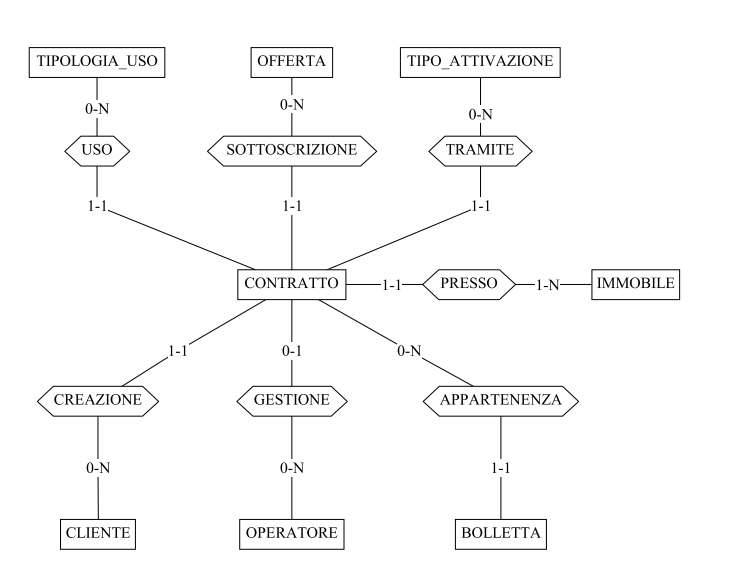
\includegraphics[width=0.9\textwidth]{images/barebones.png}}
\caption{Schema scheletro.}
\label{fig:barebones}
\end{figure}

\section{Raffinamenti proposti}
Le entità \texttt{CLIENTI} e \texttt{OPERATORI} condividono numerosi attributi, per cui si sceglie di generalizzarle creando l'entità \texttt{PERSONA} (\cref{fig:persons}). Naturalmente, si vuole impedire che uno stesso indirizzo e-mail venga usato da più individui, per cui l'attributo \texttt{Email} viene scelto come identificatore secondario di \texttt{PERSONA}.
\newline
Il \textbf{reddito} dei clienti viene modellato come entità per poter associare a ogni fascia la relativa percentuale di sconto decisa dal fornitore.

\begin{figure}[H]
\centering{}
\makebox[\textwidth][c]{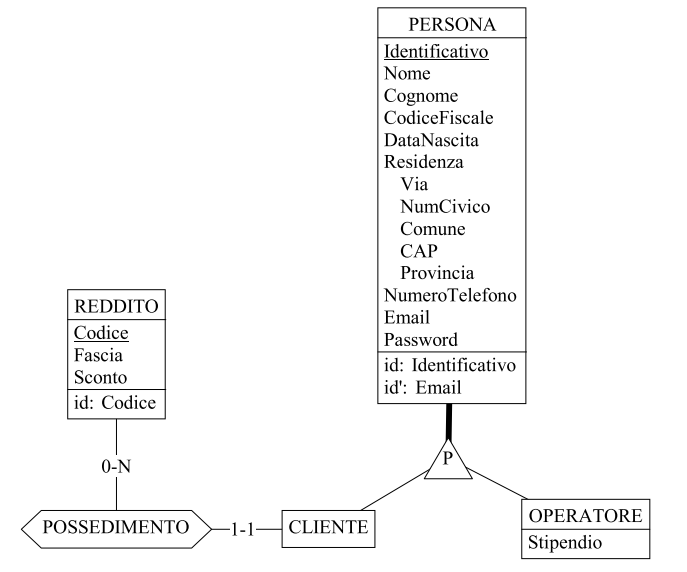
\includegraphics[width=0.71\textwidth]{images/personER.png}}
\caption{Generalizzazione di clienti e operatori.}
\label{fig:persons}
\end{figure}

In \cref{fig:plans-uses} sono rappresentate le modellazioni di offerte e tipologie d'uso. Ogni offerta è dedicata alla fornitura di una singola materia prima. Poiché nel testo è specificato che una singola offerta può essere compatibile con uno o più usi, l'associazione tra le due entità ha cardinalità molti a molti.

\begin{figure}[H]
\centering{}
\makebox[\textwidth][c]{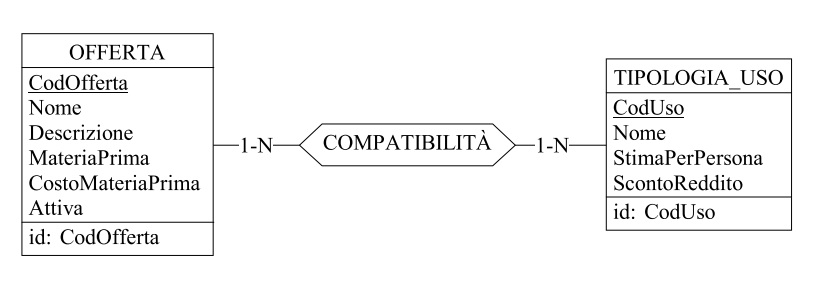
\includegraphics[width=0.7\textwidth]{images/plan-useER.png}}
\caption{Offerte e usi.}
\label{fig:plans-uses}
\end{figure}


Esistono due tipi di richieste: di \textbf{contratto} o di \textbf{cessazione}. Poiché entrambe hanno alcuni attributi in comune, si decide di modellarle per generalizzazione creando l'entità \texttt{RICHIESTA}. In \cref{fig:requests} sono inoltre rappresentate le associazioni delle richieste con clienti e operatori. Non è possibile rappresentare graficamente il fatto che lo stato di una richiesta già finalizzata non possa essere ulteriormente modificato.

\begin{figure}[H]
\centering{}
\makebox[\textwidth][c]{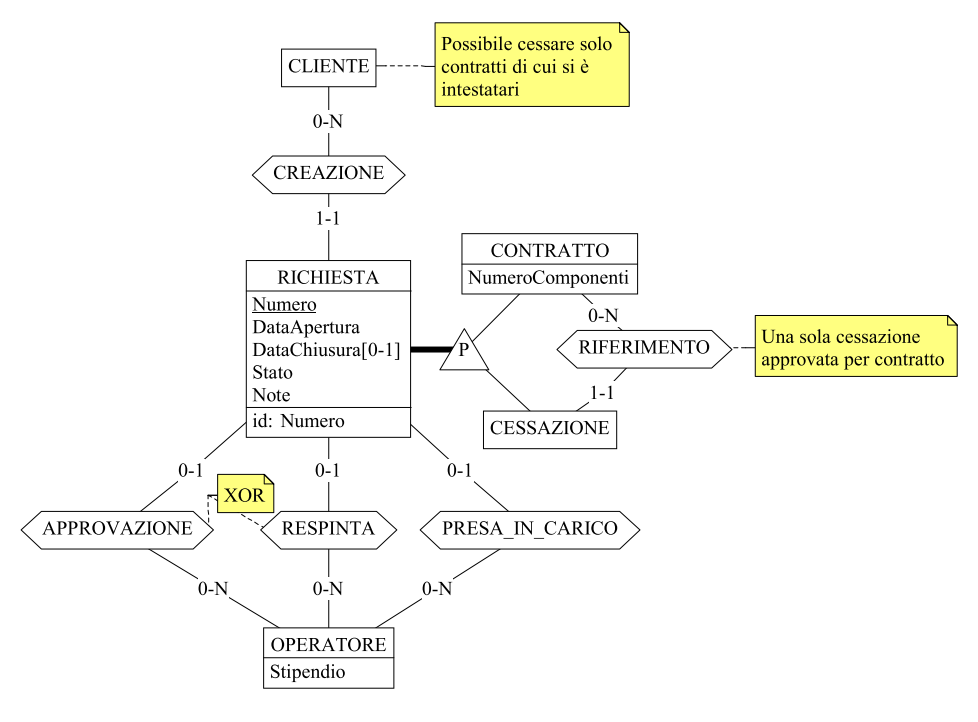
\includegraphics[width=0.8\textwidth]{images/requestER.png}}
\caption{Modellizzazione delle richieste.}
\label{fig:requests}
\end{figure}


Nella stessa figura vengono inoltre mostrate le varie associazioni che coinvolgono le due tipologie di richieste. Una richiesta di cessazione è sempre associata a un solo contratto, mentre per uno stesso contratto possono essere create più richieste di cessazione.
\newline
Vengono esplicitati testualmente i seguenti vincoli:
\begin{itemize}
    \item se esiste ed è già stata approvata una richiesta di cessazione per uno specifico contratto, non potranno essere approvate ulteriori richieste di cessazione per quel medesimo contratto
    \item un cliente non può richiedere la cessazione di contratti di cui non è intestatario
    \item l'approvazione e il rifiuto di una richiesta sono azioni mutualmente esclusive
\end{itemize}
Ciascun \textbf{tipo} di attivazione presenta un costo diverso: si decide dunque di rappresentare i tipi con l'entità \texttt{TIPO\textunderscore ATTIVAZIONE} e gli attributi in figura.\\[10pt]
In \cref{fig:requests-activation} sono rappresentate le associazioni tra contratti e offerte, tipologie d'uso e tipi di attivazione.

\begin{figure}[H]
\centering{}
\makebox[\textwidth][c]{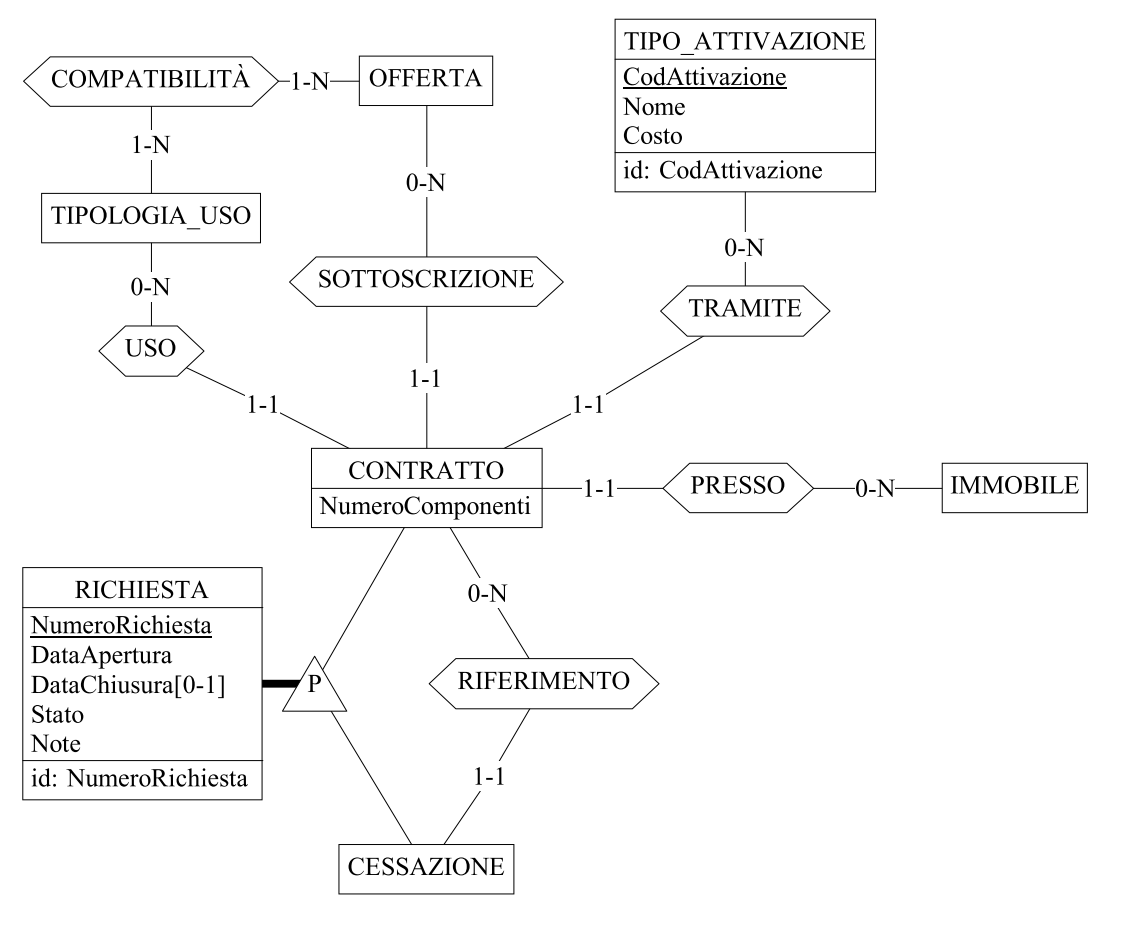
\includegraphics[width=0.8\textwidth]{images/subscription_reqER.png}}
\caption{Richieste di attivazione e di cessazione.}
\label{fig:requests-activation}
\end{figure}


In \cref{fig:meters_premises} viene mostrata la rappresentazione dei \textbf{contatori} e degli \textbf{immobili}. Un contatore è univocamente identificato dalla sua matricola o, alternativamente, dalla materia prima misurata e dall'immobile presso cui è installato; quest'ultima chiave permette di imporre il vincolo per cui in un immobile non possano essere installati più contatori misuranti la stessa materia prima.
\newline
Gli \textbf{immobili} vengono rappresentati tramite una semplice gerarchia che ne definisce il tipo.
\newline
Per quanto riguarda i \textbf{contratti}, viene esplicitato in una nota il vincolo per cui non possano esistere contemporaneamente due contratti attivi per la stessa materia prima presso un medesimo immobile.

\begin{figure}[H]
\centering{}
\makebox[\textwidth][c]{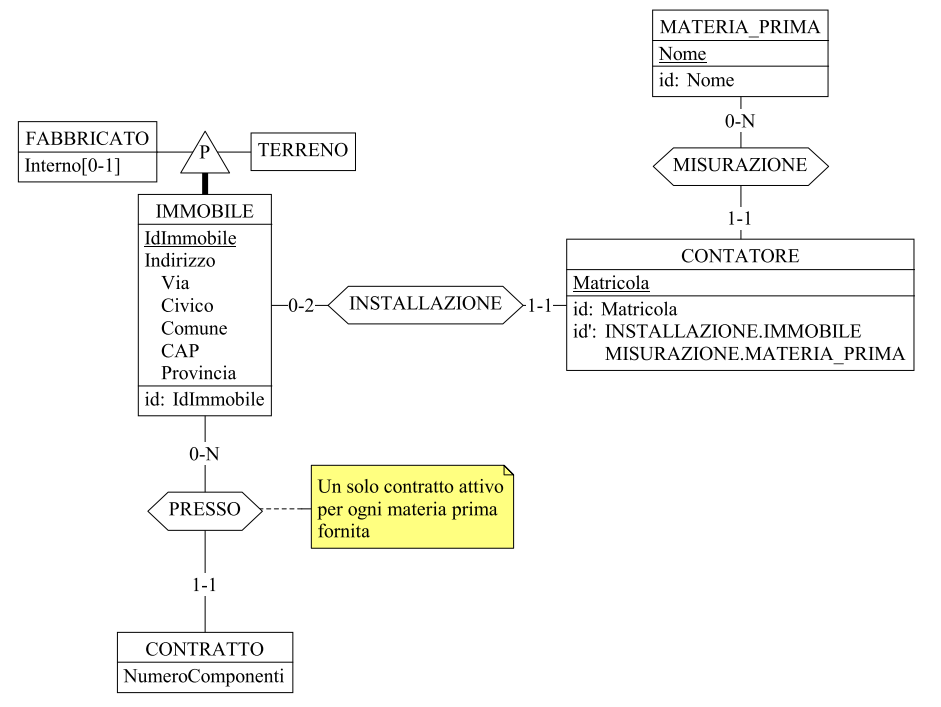
\includegraphics[width=0.9\textwidth]{images/meterER.png}}
\caption{Contatori e immobili.}
\label{fig:meters_premises}
\end{figure}


Per ogni fornitura attiva è prevista l'emissione di \textbf{bollette} (\cref{fig:reports}) con frequenza dettata dal fornitore. L'entità \texttt{BOLLETTA} presenta tutti gli attributi richiesti nelle specifiche.

\begin{figure}[H]
\centering{}
\makebox[\textwidth][c]{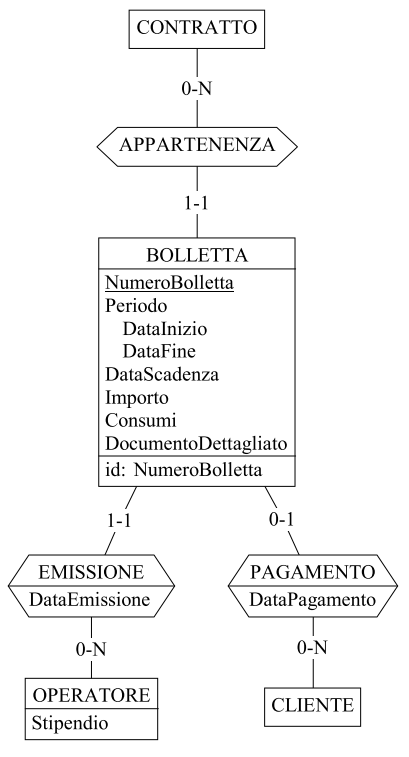
\includegraphics[width=0.4\textwidth]{images/reportER.png}}
\caption{Bollette.}
\label{fig:reports}
\end{figure}


Le \textbf{letture} (\cref{fig:measurements}) sono associate a un contatore e vengono sempre esaminate da un operatore prima di essere approvate o respinte; quest'ultimo aspetto ricorda esattamente le specifiche delle \textbf{richieste} e, dunque, nonostante non sia del tutto corretto da un punto di vista semantico, si decide di modellare l'entità \texttt{LETTURA} come specializzazione di \texttt{RICHIESTA} per evitare di ripetere una seconda volta le medesime associazioni con \texttt{OPERATORE}. Poiché è anche necessario limitare il numero di letture giornaliere a una per ogni contatore, l'attributo \texttt{DataApertura} viene spostato da \texttt{RICHIESTA} alle entità figlie (rinominato \texttt{DataEffettuazione} in \texttt{LETTURA}) e viene scelto come identificatore secondario per \texttt{LETTURA} la coppia \texttt{(DataEffettuazione, CONTATORE.Matricola)}.

\begin{figure}[H]
\centering{}
\makebox[\textwidth][c]{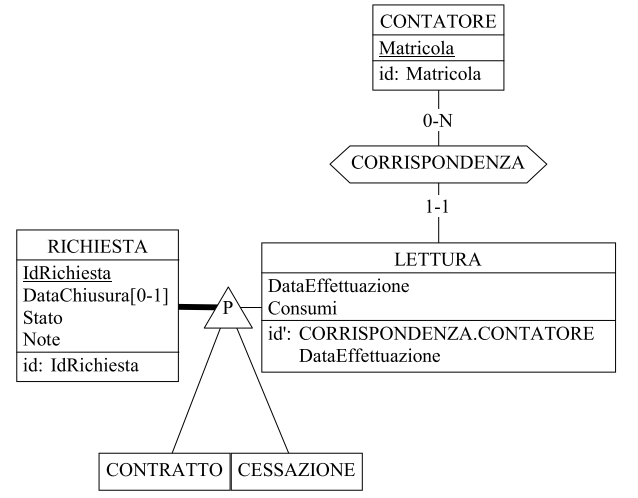
\includegraphics[width=0.7\textwidth]{images/consumpER.png}}
\caption{Letture.}
\label{fig:measurements}
\end{figure}

\section{Schema concettuale finale}
Si propone in \cref{fig:full-schema} la versione finale dello schema concettuale contenente tutte le entità e le associazioni rappresentate nei precedenti schemi parziali.

\begin{sidewaysfigure}
\centering{}
\makebox[\textwidth][c]{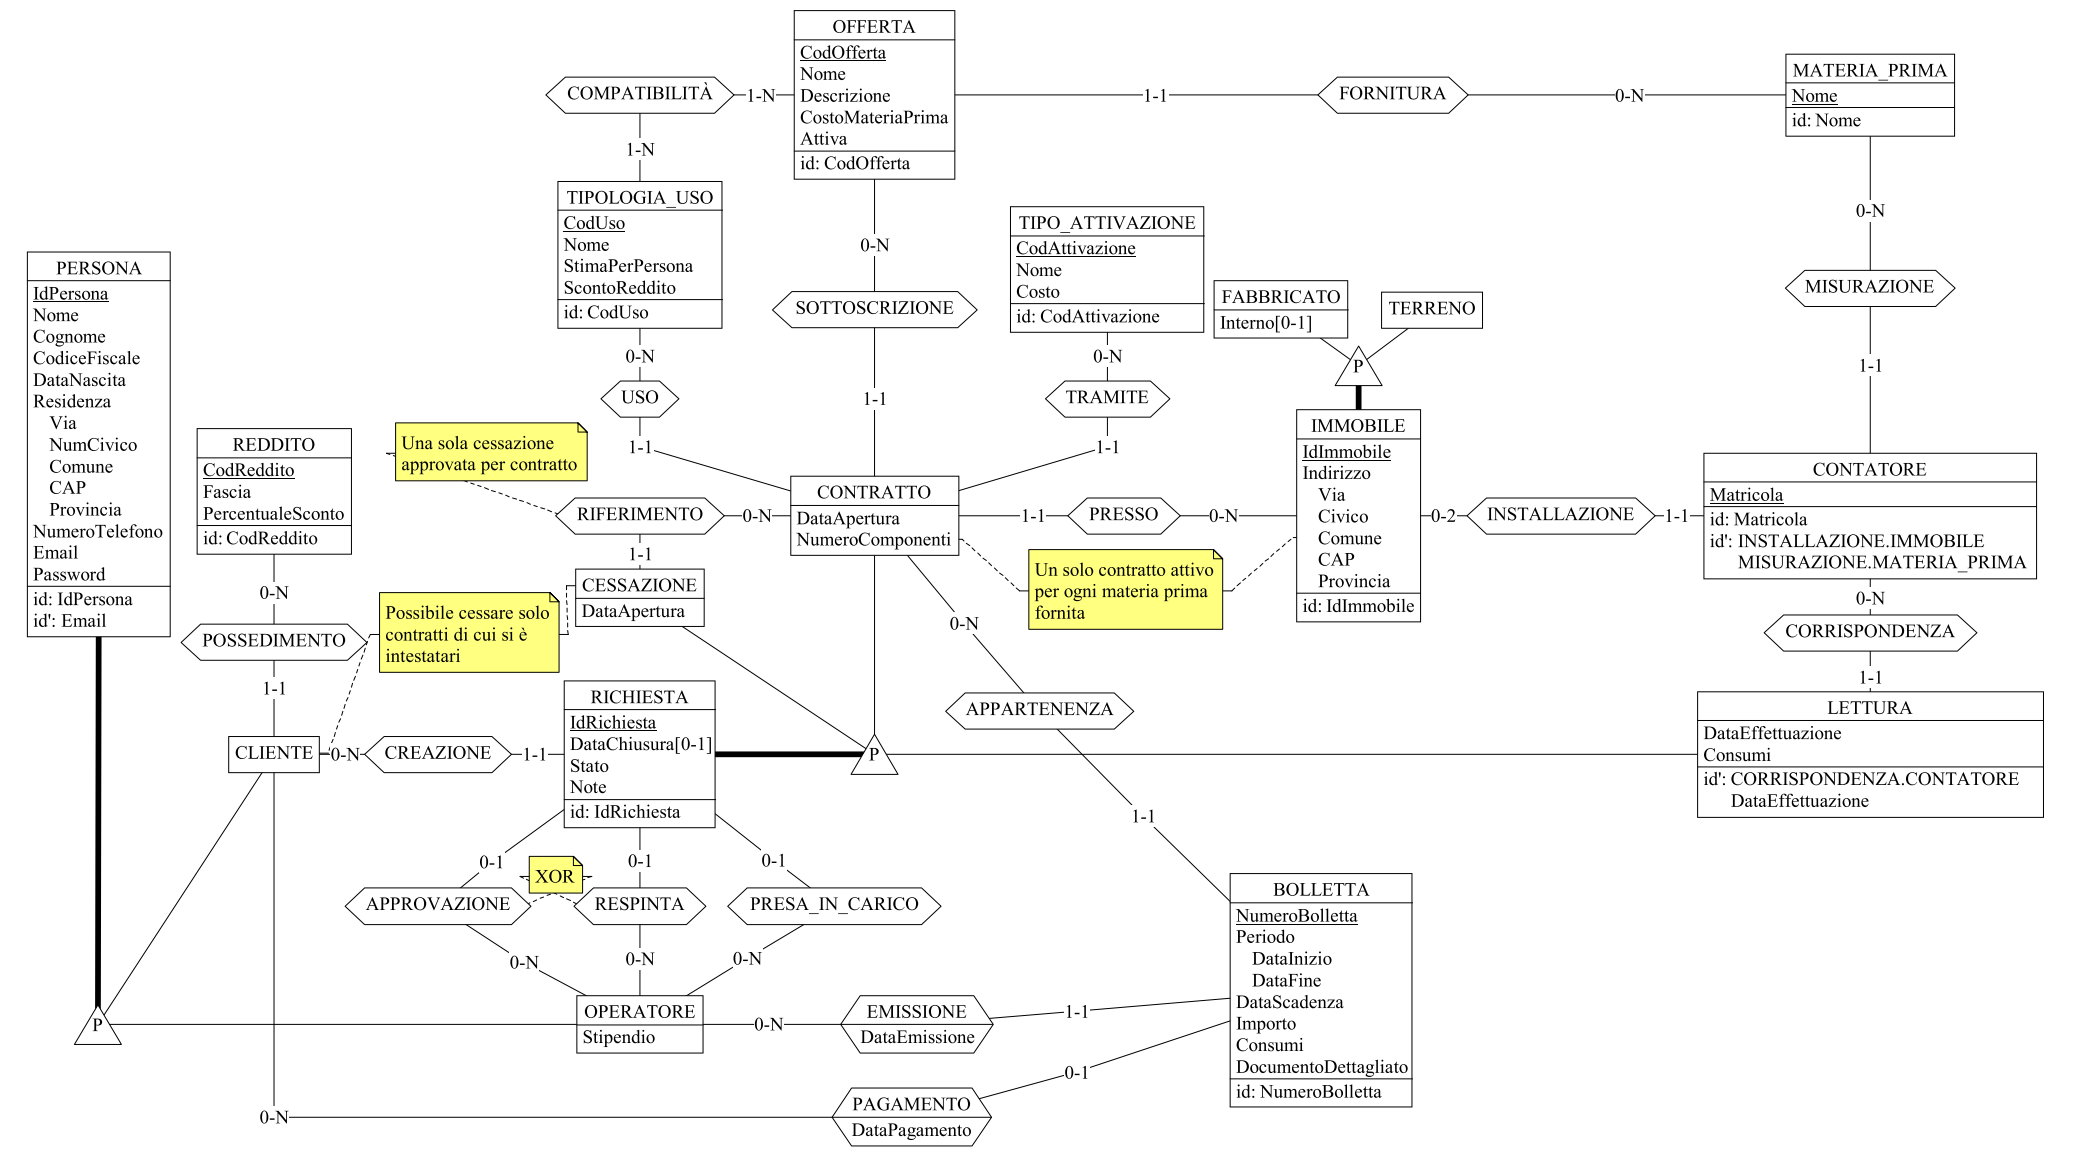
\includegraphics[width=1.0\textwidth]{images/finalER.png}}
\caption{Schema concettuale finale.}
\label{fig:full-schema}
\end{sidewaysfigure}

\chapter{Progettazione logica}
\section{Stima del volume dei dati}
 \rowcolors{1}{lightergray}{}
 \begin{longtable}{l >{\centering}p{3cm} >{\raggedleft\arraybackslash}p{4cm}}
 \hline
 \textbf{Concetto} & \textbf{Costrutto} & \textbf{Volume} \\ [0.5ex] 
 \hline
    PERSONA & \noindent{\color{blue}{E}} & 50.000 \\
    CLIENTE & \noindent{\color{blue}{E}} & 49.970 \\
    OPERATORE & \noindent{\color{blue}{E}} & 30 \\
    POSSEDIMENTO & \noindent{\color{ForestGreen}{A}} & 49.970 \\
    REDDITO & \noindent{\color{blue}{E}} & 4 \\
    CREAZIONE & \noindent{\color{ForestGreen}{A}} & 103.500 \\
    RICHIESTA & \noindent{\color{blue}{E}} & 2.000.000 \\
    CONTRATTO & \noindent{\color{blue}{E}} & 85.000 \\
    CESSAZIONE & \noindent{\color{blue}{E}} & 5.000 \\
    LETTURA & \noindent{\color{blue}{E}} & 1.910.000 \\
    CORRISPONDENZA & \noindent{\color{ForestGreen}{A}} & 1.910.000 \\
    APPROVAZIONE & \noindent{\color{ForestGreen}{A}} & 1.990.000 \\
    RESPINTA & \noindent{\color{ForestGreen}{A}} & 10.000 \\
    PRESA\textunderscore IN\textunderscore CARICO & \noindent{\color{ForestGreen}{A}} & 2.000.000 \\
    SOTTOSCRIZIONE & \noindent{\color{ForestGreen}{A}} & 90.000 \\
    OFFERTA & \noindent{\color{blue}{E}} & 15 \\
    USO & \noindent{\color{ForestGreen}{A}} & 90.000 \\
    TIPOLOGIA\textunderscore USO & \noindent{\color{blue}{E}} & 2 \\
    COMPATIBILITÀ & \noindent{\color{ForestGreen}{A}} & 23 \\
    TRAMITE & \noindent{\color{ForestGreen}{A}} & 90.000 \\
    TIPO\textunderscore ATTIVAZIONE & \noindent{\color{blue}{E}} & 3 \\
    RIFERIMENTO & \noindent{\color{ForestGreen}{A}} & 5.000 \\
    PRESSO & \noindent{\color{ForestGreen}{A}} & 85.000 \\
    CONTATORE & \noindent{\color{blue}{E}} & 70.000 \\
    IMMOBILE & \noindent{\color{blue}{E}} & 50.000 \\
    INSTALLAZIONE & \noindent{\color{ForestGreen}{A}} & 70.000 \\
    FABBRICATO & \noindent{\color{blue}{E}} & 38.000 \\
    TERRENO & \noindent{\color{blue}{E}} & 12.000 \\
    BOLLETTA & \noindent{\color{blue}{E}} & 1.000.000 \\
    EMISSIONE & \noindent{\color{ForestGreen}{A}} & 1.000.000 \\
    APPARTENENZA & \noindent{\color{ForestGreen}{A}} & 1.000.000 \\
    \hline
\end{longtable}

\section{Operazioni principali e stima della loro frequenza}
Dal testo è stata estratta una lista di possibili operazioni che verranno svolte sulla base di dati.
\\[2pt]
\rowcolors{1}{lightergray}{}
\begin{longtable}{l p{10cm} c r}
    \hline
    \textbf{Numero} & \textbf{Descrizione} & \textbf{Frequenza}\\ [0.5ex]
    \textbf{OP-1} & Inserire un nuovo cliente & 10/giorno \\
    \textbf{OP-2} & Aggiornare i dati di un cliente & 3/mese \\
    \textbf{OP-3} & Inserire un nuovo immobile & 8/giorno \\
    \textbf{OP-4} & Inserire un contatore & 10/giorno \\
    \textbf{OP-5} & Inserire una richiesta di contratto & 6/giorno \\
    \textbf{OP-6} & Selezionare l'eventuale contratto attivo intestato a un dato cliente e associato a un dato contatore (voltura) & 3/giorno \\
    \textbf{OP-7} & Selezionare l'immobile associato a un dato contatore (subentro) & 2/giorno \\
    \textbf{OP-8} & Inserire una richiesta di cessazione & 1/settimana \\
    \textbf{OP-9} & Rifiutare una richiesta & 1/giorno \\
    \textbf{OP-10} & Approvare una richiesta di contratto & 3/giorno \\
    \textbf{OP-11} & Inserire una nuova offerta & 3/mese \\
    \textbf{OP-12} & Aggiornare un'offerta & 3/mese \\
    \textbf{OP-13} & Approvare una richiesta di cessazione & 250/mese \\
    \textbf{OP-14} & Comunicare una lettura & 20.000/mese \\
    \textbf{OP-15} & Approvare una lettura & 18.000/mese \\
    \textbf{OP-16} & Rifiutare una lettura & 2.000/mese \\
    \textbf{OP-17} & Assegnare una richiesta a un operatore & 20.007/mese \\
    \textbf{OP-18} & Inserire una nuova bolletta per un contratto attivo & 235/giorno \\
    \textbf{OP-19} & Pagare una bolletta & 235/giorno \\
    \textbf{OP-20} & Visualizzare le offerte dedicate a una data materia prima e compatibili con un dato utilizzo & 1000/giorno \\
    \textbf{OP-21} & Visualizzare i contratti intestati a un dato cliente & 300/giorno \\
    \textbf{OP-22} & Visualizzare i contratti attivi intestati a un dato cliente & 300/giorno \\
    \textbf{OP-23} & Dato un contratto, visualizzare lo storico delle bollette & 1.000/mese \\
    \textbf{OP-24} & Eliminare una richiesta non finalizzata & 1/settimana \\
    \textbf{OP-25} & Visualizzare il numero di contratti stipulati in un dato anno & 3/anno \\
    \textbf{OP-26} & Visualizzare l'andamento dei consumi relativi a un contratto in un dato anno & 1.000/mese \\
    \textbf{OP-27} & Visualizzare la media dei consumi per un contratto in un dato periodo & 1.000/mese \\
    \textbf{OP-28} & Visualizzare la media aggregata dei consumi di una data materia prima prodotti in un dato periodo e relativi a tutti i contratti attivi in un dato comune & 1.000/mese \\
    \textbf{OP-29} & Visualizzare il numero di richieste di contratto finalizzate da un dato operatore & 1/mese \\
    \textbf{OP-30} & Visualizzare il numero di richieste di cessazione finalizzate da un dato operatore & 1/mese \\
    \textbf{OP-31} & Data una materia prima, visualizzare l'offerta più richiesta & 1/mese \\
    \textbf{OP-32} & Visualizzare il numero di contratti attivati in un dato anno & 1/mese \\
    \hline
\end{longtable}

\paragraph{OP-1: Inserire un nuovo cliente}\mbox{}\\
\rowcolors{1}{lightergray}{}
\begin{center}
\begin{tabular}{@{}l c  c  c@{}}
    \hline
    \textbf{Concetto} & \textbf{Costrutto} & \textbf{Accessi} & \textbf{Tipo} \\ [0.5ex]
    PERSONA & E & 1 & S \\
    CLIENTE & E & 1 & S \\
    POSSEDIMENTO & A & 1 & S \\
    \hline
\end{tabular}
\end{center}
\underline{Totale}: $3 \text{S} \times 10 = 60$ accessi al giorno 
\paragraph{OP-5: Inserire una richiesta di contratto}
\rowcolors{1}{lightergray}{}
\begin{center}
\begin{tabular}{@{}l c  c  c@{}}
    \hline
    \textbf{Concetto} & \textbf{Costrutto} & \textbf{Accessi} & \textbf{Tipo} \\ [0.5ex]
    CONTRATTO & E & 1 & S \\
    CREAZIONE & A & 1 & S \\
    USO & A & 1 & S \\
    SOTTOSCRIZIONE & A & 1 & S \\
    TRAMITE & A & 1 & S \\
    PRESSO & A & 1 & S \\
    \hline
\end{tabular}
\end{center}
\underline{Totale}: $6 \text{S} \times 6 = 72$ accessi al giorno 
\paragraph{OP-6: Selezionare l'eventuale contratto attivo intestato a un dato cliente e associato a un dato contatore (voltura)}\mbox{}\\
Per trovare il contratto attualmente attivo e procedere con la voltura, l'utente è tenuto a comunicare il codice cliente dell'attuale intestatario e la matricola del contatore.
\rowcolors{1}{lightergray}{}
\begin{center}
\begin{tabular}{@{}l c  c  c@{}}
    \hline
    \textbf{Concetto} & \textbf{Costrutto} & \textbf{Accessi} & \textbf{Tipo} \\ [0.5ex]
    CREAZIONE & A & $\frac{85.000}{49.970} = 1,17$ & L \\
    INSTALLAZIONE & A & 1 & L \\
    IMMOBILE & E & 1 & L \\
    PRESSO & A & 1 & L \\
    CONTRATTO & E & 1 & L \\
    \hline
\end{tabular}
\end{center}
\underline{Totale}: $5,17\text{L} \times 3 \simeq 15$ accessi al giorno
\paragraph{OP-11: Inserire una nuova offerta}\mbox{}\\
    Vanno specificati gli usi con cui l'offerta è compatibile e la materia prima a cui fa riferimento. Si suppone che un'offerta sia in media compatibile con una tipologia d'uso.
    \rowcolors{1}{lightergray}{}
    \begin{center}
    \begin{tabular}{@{}l c  c  c@{}}
        \hline
        \textbf{Concetto} & \textbf{Costrutto} & \textbf{Accessi} & \textbf{Tipo} \\ [0.5ex]
        OFFERTA & E & 1 & S \\
        COMPATIBILITÀ & A & 1 & S \\
        \hline
    \end{tabular}
    \end{center}
    \underline{Totale}: $2\text{S} \times 3 = 12$ accessi al mese
\paragraph{OP-13: Approvare una richiesta di cessazione}\mbox{}\\
\rowcolors{1}{lightergray}{}
\begin{center}
\begin{tabular}{@{}l c  c  c@{}}
    \hline
    \textbf{Concetto} & \textbf{Costrutto} & \textbf{Accessi} & \textbf{Tipo} \\ [0.5ex]
    CESSAZIONE & E & 1 & L \\
    CESSAZIONE & E & 1 & S \\
    \hline
\end{tabular}
\end{center}
\underline{Totale}: $(1\text{L} + 1\text{S}) \times 250 = 750$ accessi al mese
\paragraph{OP-18: Inserire una nuova bolletta per un contratto attivo}\mbox{}\\
\rowcolors{1}{lightergray}{}
\begin{center}
\begin{tabular}{@{}l c  c  c@{}}
    \hline
    \textbf{Concetto} & \textbf{Costrutto} & \textbf{Accessi} & \textbf{Tipo} \\ [0.5ex]
    RIFERIMENTO & A & $\frac{5.000}{85.000} = 0,06$ & L \\
    CESSAZIONE & E & $0,06$ & L \\
    BOLLETTA & E & 1 & S \\
    EMISSIONE & A & 1 & S \\
    APPARTENENZA & A & 1 & S \\
    \hline
\end{tabular}
\end{center}
\underline{Totale}: $(0,12\text{L} + 3\text{S}) \times 235 \simeq 1.438$ accessi al mese
\paragraph{OP-20: Visualizzare le offerte dedicate a una data materia prima e compatibili con un dato utilizzo}\mbox{}\\
    \rowcolors{1}{lightergray}{}
    \begin{center}
    \begin{tabular}{@{}l c  c  c@{}}
        \hline
        \textbf{Concetto} & \textbf{Costrutto} & \textbf{Accessi} & \textbf{Tipo} \\ [0.5ex]
        COMPATIBILITÀ & A & $\frac{23}{2} = 11$ & L \\
        OFFERTE & E & 7 & L \\
        \hline
    \end{tabular}
    \end{center}
    \underline{Totale}: $18\text{L} \times 1.000 = 180.000$ accessi al giorno
\paragraph{OP-22: Visualizzare i contratti attivi intestati a un dato cliente}\mbox{}\\
\rowcolors{1}{lightergray}{}
\begin{center}
\begin{tabular}{@{}l c  c  c@{}}
    \hline
    \textbf{Concetto} & \textbf{Costrutto} & \textbf{Accessi} & \textbf{Tipo} \\ [0.5ex]
    CREAZIONE & A & $\frac{85.000}{49.970} = 1,7$ & L \\
    CONTRATTO & E & $1,7$ & L \\
    RIFERIMENTO & A & $\frac{5.000}{85.000} = 0,06$ & L \\
    CESSAZIONE & E & $0,06$ & L \\
    \hline
\end{tabular}
\end{center}
\underline{Totale}: $3,52\text{L} \times 300 = 1.056$ accessi al giorno
\paragraph{OP-29: Visualizzare la media aggregata dei consumi relativi a tutti i contratti attivi in un dato comune}\mbox{}\\
    Per rendere meno caotico il processo di analisi, si suddivide l'operazione in due fasi.\\
    Prima di tutto, bisogna trovare tutti i contratti con una fornitura attiva nel comune di interesse. Sapendo che in Italia sono presenti 7.903 comuni e supponendo per semplicità che il numero di immobili sia uniformemente distribuito tra i comuni:
    \rowcolors{1}{lightergray}{}
    \begin{center}
    \begin{tabular}{@{}l c  c  c@{}}
        \hline
        \textbf{Concetto} & \textbf{Costrutto} & \textbf{Accessi} & \textbf{Tipo} \\ [0.5ex]
        PRESSO & A & 1 & L \\
        IMMOBILE & E & 1 & L \\
        PRESSO & A & $\frac{50.000}{7.903} = 6$ & L \\
        \hline
    \end{tabular}
    \end{center}
    Notiamo che, per ogni comune italiano, sono registrati in media circa sei immobili. Supponiamo ora che per tutti e sei gli immobili sia presente almeno un contratto (anche non attivo). In questa seconda fase ricaviamo i consumi prodotti nel periodo specificato leggendo le bollette\footnote{Non leggiamo da \texttt{LETTURA} sia perché le specifiche richiedono che vengano considerati anche i consumi stimati, sia perché il numero medio di letture per ogni contratto supera di gran lunga quello delle bollette.} emesse in quello stesso periodo.
    \rowcolors{1}{lightergray}{}
    \begin{center}
    \begin{tabular}{@{}l c  c  c@{}}
        \hline
        \textbf{Concetto} & \textbf{Costrutto} & \textbf{Accessi} & \textbf{Tipo} \\ [0.5ex]
        CONTRATTO & E & 6 & L \\
        RIFERIMENTO & A & $\frac{85.000}{5.000} \times 6 = 102$ & L \\
        BOLLETTA & E & $102$ & L \\
        \hline
    \end{tabular}
    \end{center}
    \underline{Totale}: $218\text{L} \times 1.000 = 218.000$ accessi al mese

\section{Analisi delle ridondanze}
\subsection{Attributo \texttt{Attivo} in \texttt{CONTRATTO}}
Verranno ora analizzati gli effetti dell'aggiunta all'entità \texttt{CONTRATTO} di un attributo ridondante, \texttt{Attivo}, indicante se un contratto è stato cessato o meno. Ciò permetterebbe di evitare la lettura delle eventuali cessazioni esistenti quando si considerano solo i contratti attivi.
\paragraph{OP-18 con l'uso dell'attributo ridondante}\mbox{}\\
\rowcolors{1}{lightergray}{}
\begin{center}
\begin{tabular}{@{}l c  c  c@{}}
    \hline
    \textbf{Concetto} & \textbf{Costrutto} & \textbf{Accessi} & \textbf{Tipo} \\ [0.5ex]
    CONTRATTO & E & 1 & L \\
    BOLLETTA & E & 1 & S \\
    EMISSIONE & A & 1 & S \\
    APPARTENENZA & A & 1 & S \\
    \hline
\end{tabular}
\end{center}
\underline{Totale}: $(1\text{L} + 3\text{S}) \times 235 = 1.645$ accessi al mese (contro i $1.438$ senza ridondanza)
\paragraph{OP-22 con l'uso dell'attributo ridondante}\mbox{}\\
\rowcolors{1}{lightergray}{}
\begin{center}
\begin{tabular}{@{}l c  c  c@{}}
    \hline
    \textbf{Concetto} & \textbf{Costrutto} & \textbf{Accessi} & \textbf{Tipo} \\ [0.5ex]
    CREAZIONE & A & $\frac{85.000}{49.970} = 1,7$ & L \\
    CONTRATTO & E & $1,7$ & L \\
    \hline
\end{tabular}
\end{center}
\underline{Totale}: $3,4\text{L} \times 300 = 1.020$ accessi al giorno (contro i $1.056$ senza ridondanza)
\\[10pt]
In termini di accessi, si ha un beneficio quasi trascurabile in OP-18 e un leggerissimo peggioramento in OP-22; pertanto, si decide di non aggiungere l'attributo \texttt{Attivo}.

\section{Raffinamento dello schema}
\subsection{Eliminazione delle gerarchie}
\begin{itemize}
    \item Le entità \texttt{CLIENTE} e \texttt{OPERATORE}, entrambe specializzazioni di \texttt{PERSONA}, hanno ruoli diametralmente opposti e si relazionano alle altre entità con associazioni tutte diverse. Poiché la loro copertura è totale ed esclusiva, avrebbe senso procedere con un collasso verso il basso, ma ciò significherebbe anche replicare la grande quantità di attributi di \texttt{PERSONA} in due relazioni diverse e costringerebbe a effettuare controlli aggiuntivi per evitare che i dati di una stessa persona compaiano in entrambe le relazioni. Si preferisce, dunque, effettuare una trasformazione per associazioni: \texttt{CLIENTE} e \texttt{OPERATORE} vengono associati a \texttt{PERSONA} e da essa ricaveranno la chiave primaria e tutti gli altri attributi. Dovremo solo assicurarci che lo stesso codice identificativo di una persona venga inserito o solo in \texttt{CLIENTE} o solo in \texttt{OPERATORE}.
    \item Le specializzazioni di \texttt{IMMOBILE} non hanno associazioni con altre entità del dominio, per cui si procede con una trasformazione verso l'alto aggiungendo a \texttt{IMMOBILE} gli attributi \texttt{Tipo} e \texttt{Interno}.
    \item Per la gerarchia di \texttt{RICHIESTA} si procede con una trasformazione verso il basso: l'entità \texttt{RICHIESTA} viene eliminata e i suoi attributi integrati in \texttt{CONTRATTO}, \texttt{CESSAZIONE} e \texttt{LETTURA}.
\end{itemize}

\subsection{Eliminazione degli attributi multivalore}
I seguenti attributi multivalore sono stati eliminati e le loro componenti disaggregate:
\begin{itemize}
    \item \texttt{Residenza}, dell'entità \texttt{PERSONA}
    \item \texttt{Indirizzo}, dell'entità \texttt{IMMOBILE}
    \item \texttt{Periodo}, dell'entità \texttt{BOLLETTA}
\end{itemize}

\subsection{Scelta delle chiavi}
\begin{itemize}
    \item \texttt{CLIENTE} e \texttt{OPERATORE} vengono identificati rispettivamente dalle chiavi esterne \texttt{CodiceCliente} e \texttt{IdOperatore}, che fanno riferimento alla chiave \texttt{IdPersona} di \texttt{PERSONA}
    \item \texttt{CONTRATTO} e \texttt{CESSAZIONE} hanno ora una propria chiave primaria, \texttt{IdRichiesta}
    \item \texttt{LETTURA} viene identificata dall'attributo \texttt{NumeroLettura}
    \item Si aggiunge una chiave candidata a \texttt{IMMOBILE} composta da tutti gli attributi tranne \texttt{IdImmobile}
\end{itemize}

\subsection{Eliminazione degli identificatori esterni}
Si procede alla trasformazione delle associazioni:
\begin{itemize}
    \item \texttt{POSSEDIMENTO} viene eliminata e la chiave esterna \texttt{FasciaReddito} aggiunta a \texttt{CLIENTE}
    \item \texttt{CREAZIONE} viene eliminata e la chiave esterna \texttt{IdCliente} aggiunta a \texttt{RICHIESTA}
    \item \texttt{PRESA\textunderscore IN \textunderscore CARICO} viene reificata. All'atto della creazione, una richiesta non risulta assegnata ad alcun operatore e contiene quindi un riferimento nullo a \texttt{OPERATORE}; per evitare ciò, gli assegnamenti delle richieste ai vari operatori verranno inseriti in tre relazioni distinte (\texttt{OPERATORI\textunderscore CESSAZIONI}, \texttt{OPERATORI\textunderscore CONTRATTI} e \texttt{OPERATORI\textunderscore LETTURE}), ognuna dedicata a una diversa tipologia di richiesta
    \item \texttt{APPROVATA} e \texttt{RESPINTA} vengono eliminate
    \item \texttt{USO} viene eliminata e la chiave esterna \texttt{Uso} aggiunta a \texttt{CONTRATTO}
    \item \texttt{SOTTOSCRIZIONE} viene eliminata e la chiave esterna \texttt{Offerta} aggiunta all'entità \texttt{CONTRATTO}
    \item \texttt{TRAMITE} viene eliminata e la chiave esterna \texttt{TipoAttivazione} aggiunta all'entità \texttt{CONTATTO}
    \item \texttt{PRESSO} viene eliminata e la chiave esterna \texttt{IdImmobile} aggiunta all'entità \texttt{CONTRATTO}
    \item \texttt{APPARTENENZA} viene eliminata e la chiave esterna \texttt{IdContratto} aggiunta all'entità \texttt{BOLLETTA}
    \item \texttt{EMISSIONE} viene eliminata e la chiave esterna \texttt{IdOperatore} importata nell'entità \texttt{BOLLETTA}
    \item \texttt{PAGAMENTO} viene reificata per evitare di aggiungere il campo opzionale \texttt{DataPagamento} in \texttt{BOLLETTA}; le tuple di \texttt{PAGAMENTO} conterranno, per le bollette saldate, una bolletta e la relativa data di pagamento
    \item \texttt{CORRISPONDENZA} viene eliminata e la chiave esterna \texttt{MatricolaContatore} aggiunta a \texttt{LETTURA}
    \item \texttt{INSTALLAZIONE} viene eliminata e la chiave esterna \texttt{IdImmobile} aggiunta a \texttt{CONTATORE}
    \item \texttt{COMPATIBILITÀ} viene reificata come traduzione di un'associazione molti a molti; le sue istanze conterranno un'offerta e una tipologia d'uso
\end{itemize}

\section{Traduzione di entità e associazioni in relazioni}
\begin{itemize}
    \item \texttt{BOLLETTE(\underline{NumeroBolletta}, DataEmissione, DataInizioPeriodo, DataFinePeriodo, DataScadenza, Importo, Consumi, DocumentoDettagliato, IdOperatore, IdContratto) \\
    FK: IdOperatore REFERENCES OPERATORI \\
    FK: IdContratto REFERENCES CONTRATTI}
    
    \item \texttt{CESSAZIONI(\underline{NumeroRichiesta}, DataAperturaRichiesta, DataChiusuraRichiesta*, StatoRichiesta, NoteRichiesta, IdContratto) \\
    FK: IdContratto REFERENCES CONTRATTI}
    
    \item \texttt{CLIENTI(\underline{CodiceCliente}, FasciaReddito) \\
    FK: CodiceCliente REFERENCES PERSONE \\
    FK: FasciaReddito REFERENCES REDDITI}
    
    \item \texttt{COMPATIBILITÀ(\underline{Offerta}, \underline{Uso}) \\
    FK: Offerta REFERENCES OFFERTE \\
    FK: Uso REFERENCES TIPOLOGIE\textunderscore USO
    }
    
    \item \texttt{CONTATORI(\underline{Matricola}, MateriaPrima, IdImmobile) \\
    UNIQUE(IdImmobile, MateriaPrima) \\
    FK: IdImmobile REFERENCES IMMOBILI}
    
    \item \texttt{CONTRATTI(\underline{IdContratto}, DataAperturaRichiesta, DataChiusuraRichiesta*, StatoRichiesta, NoteRichiesta, NumeroComponenti, Uso, Offerta, TipoAttivazione, IdImmobile, IdCliente) \\
    FK: Uso REFERENCES TIPOLOGIE\textunderscore USI \\
    FK: Offerta REFERENCES OFFERTE \\
    FK: TipoAttivazione REFERENCES TIPI\textunderscore ATTIVAZIONE \\
    FK: IdImmobile REFERENCES IMMOBILI \\
    FK: IdCliente REFERENCES CLIENTI}
    
    \item \texttt{IMMOBILI(\underline{IdImmobile}, Tipo, Via, NumCivico, Interno, Comune, CAP, Provincia) \\
    UNIQUE(Tipo, Via, NumCivico, Interno, Comune, CAP, Provincia)}
    
    \item \texttt{LETTURE(\underline{NumeroLettura}, MatricolaContatore, DataEffettuazione, Consumi, Stato, IdCliente) \\
    UNIQUE(MatricolaContatore, DataEffettuazione) \\
    FK: IdCliente REFERENCES CLIENTI \\
    FK: MatricolaContatore REFERENCES CONTATORI}
    
    \item \texttt{OFFERTE(\underline{CodOfferta}, Nome, Descrizione, MateriaPrima, CostoMateriaPrima, Attiva)}
    
    \item \texttt{OPERATORI(\underline{IdOperatore}, Stipendio) \\
    FK: IdOperatore REFERENCES PERSONE}
    
    \item \texttt{OPERATORI\textunderscore CESSAZIONI(\underline{NumeroRichiesta}, IdOperatore) \\
    FK: NumeroRichiesta REFERENCES CESSAZIONI \\
    FK: IdOperatore REFERENCES OPERATORI}
    
    \item \texttt{OPERATORI\textunderscore CONTRATTI(\underline{NumeroRichiesta}, IdOperatore) \\
    FK: NumeroRichiesta REFERENCES CONTRATTI \\
    FK: IdOperatore REFERENCES OPERATORI}
    
    \item \texttt{OPERATORI\textunderscore LETTURE(\underline{Lettura}, IdOperatore) \\
    FK: Lettura REFERENCES LETTURE \\
    FK: IdOperatore REFERENCES OPERATORE}
    
    \item \texttt{PAGAMENTI(\underline{NumeroBolletta}, DataPagamento) \\
    FK: NumeroBolletta REFERENCES BOLLETTE}
    
    \item \texttt{PERSONE(\underline{IdPersona}, Nome, Cognome, CodiceFiscale, DataNascita, Via, NumCivico, Comune, CAP, Provincia, NumeroTelefono, Email, Password) \\
    UNIQUE(Email)}
    
    \item \texttt{REDDITI(\underline{CodReddito}, Fascia, Sconto)}
    
    \item \texttt{TIPI\textunderscore ATTIVAZIONE(\underline{CodAttivazione}, Nome, Costo)}
    
    \item \texttt{TIPOLOGIE\textunderscore USO(\underline{CodUso}, Nome, StimaPerPersona, ScontoReddito)}
\end{itemize}

\section{Schema relazionale finale}
In \cref{fig:full-relational} viene proposto lo schema relazionale finale.

\begin{sidewaysfigure}
\centering{}
\makebox[\textwidth][c]{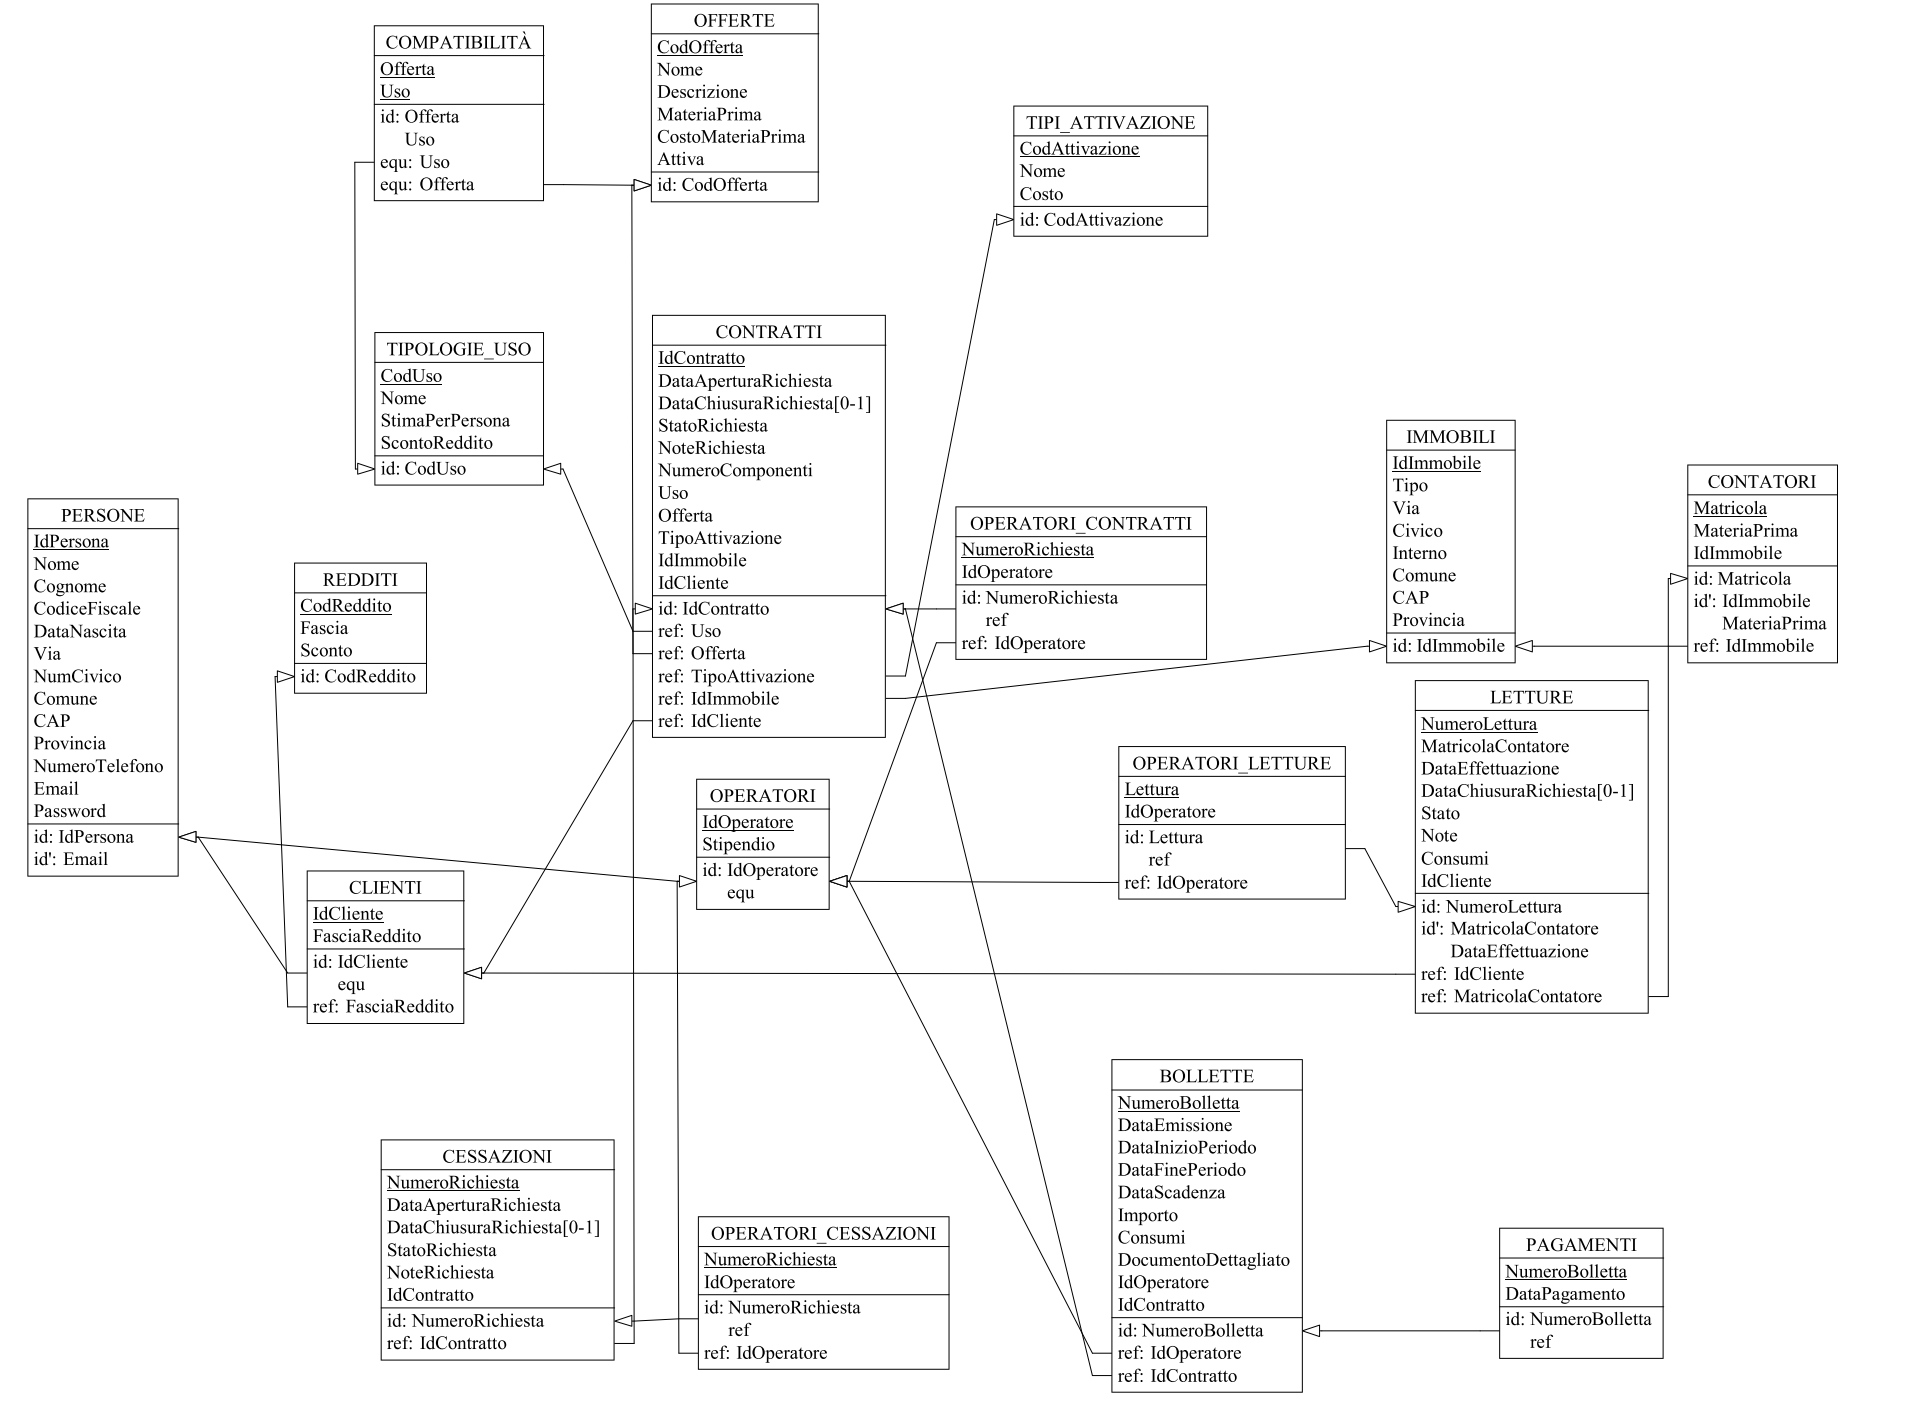
\includegraphics[width=0.9\textwidth]{images/relational.png}}
\caption{Schema relazionale finale.}
\label{fig:full-relational}
\end{sidewaysfigure}
\newpage
\section{Traduzione delle operazioni in query SQL}
\paragraph{OP-1: Inserire un nuovo cliente}\mbox{}\\
\begin{lstlisting}
insert into persone
values (default, ?, ?, ?, ?, ?, ?, ?, ?, ?, ?, ?, ?);

insert into clienti
values (last_insert_id(), ?);
\end{lstlisting}

\paragraph{OP-2: Aggiornare i dati di un cliente}\mbox{}\\
\begin{lstlisting}
update persone
set Email = ?, Cap = ?, Comune = ?, NumCivico = ?, NumeroTelefono = ?, Provincia = ?, Via = ?
where IdPersona = ?;
\end{lstlisting}
    
\paragraph{OP-3: Inserire un nuovo immobile}\mbox{}\\
\begin{lstlisting}
insert into immobili (Tipo, Via, NumCivico, Interno, Comune, CAP, Provincia)
values (?, ?, ?, ?, ?, ?, ?);
\end{lstlisting}
    
\paragraph{OP-4: Inserire un contatore}\mbox{}\\
\begin{lstlisting}
insert into contatori
values (?, ?, ?);
\end{lstlisting}

\paragraph{OP-5: Inserire una richiesta di contratto}\mbox{}\\
\begin{lstlisting}
insert into contratti (DataAperturaRichiesta, StatoRichiesta, NoteRichiesta, Offerta, Uso, TipoAttivazione, NumeroComponenti, IdImmobile, IdCliente)
values (curdate(), "In lavorazione", "", ?, ?, ?, ?, ?, ?);
\end{lstlisting}

\paragraph{OP-6: Selezionare l'eventuale contratto attivo intestato a un dato cliente e associato a un dato contatore (voltura)}\mbox{}\\
\begin{lstlisting}
select C.*
from `contratti attivi` C, immobili I, contatori M, offerte O
where C.IdCliente = ?
and C.IdImmobile = I.IdImmobile
and I.IdImmobile = M.IdImmobile
and M.Matricola = ?
and C.Offerta = O.CodOfferta
and O.MateriaPrima = M.MateriaPrima;
\end{lstlisting}

\paragraph{OP-7: Selezionare l'immobile associato a un dato contatore (subentro)}\mbox{}\\
\begin{lstlisting}
select immobili.*
from immobili, contatori
where contatori.Matricola = ?
and contatori.IdImmobile = immobili.IdImmobile;
\end{lstlisting}

\paragraph{OP-8: Inserire una richiesta di cessazione}\mbox{}\\
\begin{lstlisting}
insert into cessazioni (IdContratto, DataAperturaRichiesta, StatoRichiesta, NoteRichiesta)
values (?, curdate(), "In lavorazione", ?, "");
\end{lstlisting}

\paragraph{OP-9: Rifiutare una richiesta}\mbox{}\\
L'operazione va a buon fine se l'operatore che sta rifiutando la richiesta è lo stesso che l'ha presa in carico.
\begin{lstlisting}
-- In caso di richiesta di contratto
update contratti
set StatoRichiesta = "Respinta", DataChiusuraRichiesta = curdate(), NoteRichiesta = ?
where IdContratto = ?
and StatoRichiesta = "In lavorazione"
and DataChiusuraRichiesta is null
and exists (select *
            from `operatori contratti` OC
            where OC.NumeroRichiesta = ?
            and OC.IdOperatore = ?)

-- In caso di richiesta di cessazione
update cessazioni
set StatoRichiesta = "Respinta", DataChiusuraRichiesta = curdate(), NoteRichiesta = ?
where NumeroRichiesta = ?
and StatoRichiesta = "In lavorazione"
and DataChiusuraRichiesta is null
and exists (select *
            from `operatori cessazioni` OC
            where OC.NumeroRichiesta = ?
            and OC.IdOperatore = ?)
\end{lstlisting}

\paragraph{OP-10: Approvare una richiesta di contratto}\mbox{}\\
La richiesta viene approvata se 
\begin{itemize}
    \item per l'immobile non esiste già un contratto attivo per la stessa materia prima
    \item se l'immobile possiede un contatore adatto per la materia prima scelta
    \item se l'operatore che sta approvando la richiesta è lo stesso che l'ha presa in carico
\end{itemize}
\begin{lstlisting}
update contratti
set DataChiusuraRichiesta = curdate(), StatoRichiesta = "Approvata", NoteRichiesta = :notes
where IdContratto = :requestId
and StatoRichiesta = "In lavorazione"
and DataChiusuraRichiesta is null
and exists (select *
            from `operatori contratti` OC
            where OC.NumeroRichiesta = ?
            and OC.IdOperatore = ?)
and exists (select M.Matricola
            from contratti C, immobili I, contatori M, offerte O
            where C.IdContratto = :requestId
            and I.IdImmobile = C.IdImmobile
            and M.IdImmobile = I.IdImmobile
            and O.CodOfferta = C.Offerta
            and O.MateriaPrima = M.MateriaPrima)
and not exists (select C.IdContratto
                from contratti C, immobili I, offerte O, contatori M
                where I.IdImmobile = (select distinct(C2.IdImmobile)
                                    from contratti C2
                                    where C2.IdContratto = :requestId)
                and C.IdImmobile = I.IdImmobile
                and M.IdImmobile = I.IdImmobile
                and O.CodOfferta = C.Offerta
                and O.MateriaPrima = M.MateriaPrima
                and C.StatoRichiesta = "Approvata"
                and C.DataChiusuraRichiesta is not null
                and not exists (select E.NumeroRichiesta
                                from cessazioni E
                                where E.IdContratto = C.IdContratto
                                and E.DataChiusuraRichiesta is not null
                                and E.StatoRichiesta = "Approvata"));
\end{lstlisting}

\paragraph{OP-11: Inserire una nuova offerta}\mbox{}\\
\begin{lstlisting}
insert into offerte
values (default, ?, ?, ?, ?, ?);

-- Ripetere per ogni uso con cui si vuole rendere compatibile l'offerta
insert into compatibilità
values (last_insert_id(), ?);
\end{lstlisting}
    
\paragraph{OP-12: Aggiornare un'offerta}\mbox{}\\
\begin{lstlisting}
update offerte
set Nome = ?, Descrizione = ?, CostoMateriaPrima = ?, Attiva = ?, MateriaPrima = ?
where CodOfferta = ?;
\end{lstlisting}

\paragraph{OP-13: Approvare una richiesta di cessazione}\mbox{}\\
La richiesta viene approvata se non esiste un'altra richiesta di cessazione già approvata per lo stesso contratto.
\begin{lstlisting}
update cessazioni
set StatoRichiesta = "Approvata", NoteRichiesta = :notes, DataChiusuraRichiesta = curdate()
where cessazioni.NumeroRichiesta = :requestId
and cessazioni.StatoRichiesta = "In lavorazione"
and cessazioni.DataChiusuraRichiesta is null
and exists (select *
            from `operatori cessazioni` OC
            where OC.NumeroRichiesta = ?
            and OC.IdOperatore = ?)
and not exists (select C.NumeroRichiesta
                from cessazioni C
                where C.IdContratto = (select C2.IdContratto
                                        from cessazioni C2
                                        where C2.NumeroRichiesta = :requestId)
                and C.StatoRichiesta = "Approvata"
                and C.DataChiusuraRichiesta is not null)
\end{lstlisting}

\paragraph{OP-14: Comunicare una lettura}\mbox{}\\
All'inserimento di ogni lettura bisogna verificare che il cliente abbia un contratto attivo associato al contatore e che i consumi rilevati siano maggiori di quelli riportati nell'ultima lettura salvata. Se si comunicano più letture nello stesso giorno, viene mantenuta solo quella più recente.
\begin{lstlisting}
insert into letture (MatricolaContatore, DataEffettuazione, Consumi, Stato, Note, IdCliente)
select :meterId, curdate(), :consumption, "In lavorazione", "", :clientId
where exists (select CA.IdContratto
            from `contratti attivi` CA, contatori C, immobili I, offerte O
            where C.Matricola = :meterId
            and C.IdImmobile = I.IdImmobile
            and I.IdImmobile = CA.IdImmobile
            and CA.IdCliente = :clientId
            and CA.Offerta = O.CodOfferta
            and O.MateriaPrima = C.MateriaPrima)
and (not exists (select L.Consumi
                from letture L
                where L.MatricolaContatore = :meterId
                and L.Stato = "Approvata"
                and L.DataChiusuraRichiesta is not null
                order by L.DataEffettuazione desc
                limit 1)
    or (select L.Consumi
        from letture L
        where L.MatricolaContatore = :meterId
        and L.Stato = "Approvata"
        and L.DataChiusuraRichiesta is not null
        order by L.DataEffettuazione desc
        limit 1) <= :consumption)
on duplicate key update letture.Consumi = case when letture.Stato = "In lavorazione" then :consumption else letture.Consumi end;
\end{lstlisting}

\paragraph{OP-15: Approvare una lettura}\mbox{}\\
L'operazione va a buon fine se l'operatore che sta approvando la lettura è lo stesso che l'ha presa in carico.
\begin{lstlisting}
update letture
set Stato = "Approvata", DataChiusuraRichiesta = curdate(), Note = ?
where NumeroLettura = ?;
and Stato = "In lavorazione"
and DataChiusuraRichiesta is null
and exists (select *
            from `operatori letture` OL
            where OL.Lettura = ?
            and OL.IdOperatore = ?);
\end{lstlisting}

\paragraph{OP-16: Rifiutare una lettura}\mbox{}\\
L'operazione va a buon fine se l'operatore che sta rifiutando la lettura è lo stesso che l'ha presa in carico.
\begin{lstlisting}
update letture
set Stato = "Respinta", DataChiusuraRichiesta = curdate(), Note = ?
where NumeroLettura = ?
and Stato = "In lavorazione"
and DataChiusuraRichiesta is null
and exists (select *
            from `operatori letture` OL
            where OL.Lettura = ?
            and OL.IdOperatore = ?);
\end{lstlisting}

\paragraph{OP-17: Assegnare una richiesta a un operatore}\mbox{}\\
\begin{lstlisting}
-- In caso di richiesta di contratto
insert into `operatori contratti`
vaules (?, ?)
on duplicate key ignore;


-- In caso di richiesta di cessazione
insert into `operatori cessazioni`
vaules (?, ?)
on duplicate key ignore;
\end{lstlisting}
    
\paragraph{OP-18: Inserire una nuova bolletta per un contratto attivo}\mbox{}\\
\begin{lstlisting}
insert into bollette (DataEmissione, DataInizioPeriodo, DataFinePeriodo, DataScadenza, Importo, Consumi, DocumentoDettagliato, IdOperatore, IdContratto)
select curdate(), :intervalStartDate, :intervalEndDate, :deadline, :finalCost, :consumption, :reportFile, :operatorId, :subId
from `contratti attivi`
where `contratti attivi`.IdContratto = :subId;
\end{lstlisting}

\paragraph{OP-19: Pagare una bolletta}\mbox{}\\
\begin{lstlisting}
insert into pagamenti
values (?, curdate())
on duplicate key ignore;
\end{lstlisting}

\paragraph{OP-20: Visualizzare le offerte dedicate a una data materia prima e compatibili con un dato utilizzo}\mbox{}\\
\begin{lstlisting}
select O.*
from offerte O, compatibilità C
where O.MateriaPrima = ?
and O.Attiva = true
and C.Uso = ?
and O.CodOfferta = C.Offerta;
\end{lstlisting}

\paragraph{OP-21: Visualizzare i contratti intestati a un dato cliente}\mbox{}\\
\begin{lstlisting}
select C.*
from `contratti approvati` C
where C.IdCliente = ?;
\end{lstlisting}

\paragraph{OP-22: Visualizzare i contratti attivi intestati a un dato cliente}\mbox{}\\
\begin{lstlisting}
select C.*
from `contratti attivi` C
where C.IdCliente = ?;
\end{lstlisting}

\paragraph{OP-23: Dato un contratto, visualizzare lo storico delle bollette}\mbox{}\\
\begin{lstlisting}
select *
from bollette
where bollette.IdContratto = ?;
\end{lstlisting}

\paragraph{OP-24: Eliminare una richiesta non finalizzata}\mbox{}\\
\begin{lstlisting}
-- In caso di richiesta di contratto
delete contratti
where IdContratto = ?
and StatoRichiesta = "In lavorazione"
and DataChiusuraRichiesta is null;

-- In caso di richiesta di cessazione
delete cessazioni
where NumeroRichiesta = ?
and StatoRichiesta = "In lavorazione"
and DataChiusuraRichiesta is null;
\end{lstlisting}

\paragraph{OP-25: Visualizzare il numero di contratti stipulati in un dato anno}\mbox{}\\
\begin{lstlisting}
select count(C.IdContratto) as NumeroContratti
from `contratti approvati` C
where year(C.DataChiusuraRichiesta) = ?;
\end{lstlisting}

\paragraph{OP-26: Visualizzare l'andamento dei consumi relativi a un contratto in un dato anno}\mbox{}\\
\begin{lstlisting}
select B.DataFinePeriodo, B.Consumi
from bollette B
where B.IdContratto = ?
and year(B.DataFinePeriodo) = ?;
\end{lstlisting}

\paragraph{OP-27: Visualizzare la media dei consumi per un contratto in un dato periodo}\mbox{}\\
\begin{lstlisting}
select avg(B.Consumi) as MediaContratto
from bollette B, `contratti approvati` C
where C.IdContratto = ?
and B.IdContratto = C.IdContratto
and B.DataFinePeriodo between ? and ?;
\end{lstlisting}

\paragraph{OP-28: Visualizzare la media aggregata dei consumi di una data materia prima prodotti in un dato periodo e relativi a tutti i contratti attivi in un dato comune}\mbox{}\\
\begin{lstlisting}
select avg(B.Consumi) as MediaComune
from bollette B, `contratti approvati` C, immobili I, offerte O
where O.MateriaPrima = ?
and C.Offerta = O.CodOfferta
and I.Comune = ?
and I.Provincia = ?
and C.IdImmobile = I.IdImmobile
and C.IdContratto = B.IdContratto
and B.DataFinePeriodo between ? and ?;
\end{lstlisting}

\paragraph{OP-29: Visualizzare il numero di richieste di contratto finalizzate da un dato operatore}\mbox{}\\
\begin{lstlisting}
select count(*) as RichiesteTotali
from `operatori contratti` OC, contratti C
where OC.NumeroRichiesta = C.IdContratto
and OC.IdOperatore = ?
and C.StatoRichiesta != "In lavorazione"
and C.DataChiusuraRichiesta is not null;
\end{lstlisting}

\paragraph{OP-30: Visualizzare il numero di richieste di cessazione finalizzate da un dato operatore}\mbox{}\\
\begin{lstlisting}
select count(*) as RichiesteTotali
from `operatori cessazioni` OC, cessazioni C
where OC.NumeroRichiesta = C.NumeroRichiesta
and OC.IdOperatore = ?
and C.StatoRichiesta != "In lavorazione"
and C.DataChiusuraRichiesta is not null;
\end{lstlisting}

\paragraph{OP-31: Data una materia prima, visualizzare l'offerta più richiesta}\mbox{}\\
\begin{lstlisting}
select O.CodOfferta, O.Nome, count(C.IdContratto) as NumeroContratti
from offerte O, contratti C
where C.Offerta = O.CodOfferta
group by O.CodOfferta
order by NumeroContratti desc
limit 1;

\end{lstlisting}

\paragraph{OP-32: Visualizzare il numero di contratti attivati in un dato anno}\mbox{}\\
\begin{lstlisting}
select count(*)
from `contratti approvati` C
where year(C.DataChiusuraRichiesta) = ?;
\end{lstlisting}

\chapter{Progettazione dell'applicazione}
Per lo sviluppo dell'applicazione si è scelto come DBMS di riferimento \textbf{MySQL}. Il front-end, sviluppato in Java, segue il pattern architetturale MVC e utilizza la libreria grafica \textbf{JavaFX}. Per la comunicazione col database si è optato per la libreria \textbf{jOOQ}, la quale offre un più alto livello di astrazione rispetto alla API JDBC. La gestione delle librerie è stata agevolata dall'utilizzo del sistema di build automation \textbf{Gradle}.
\newline
L'applicazione si presenta all'avvio con una schermata in cui è possibile consultare liberamente il catalogo delle offerte, effettuare l'accesso oppure, se non lo si è già fatto, registrarsi. Clienti e operatori hanno accesso a zone diverse dell'applicazione: ad esempio, l'accesso all'area clienti (\cref{fig:user-area}) e al catalogo pubblico non è permesso agli operatori, che, come da specifiche, non possono sottoscrivere contratti col fornitore.

\begin{figure}[H]
    \centering{}
    \makebox[\textwidth][c]{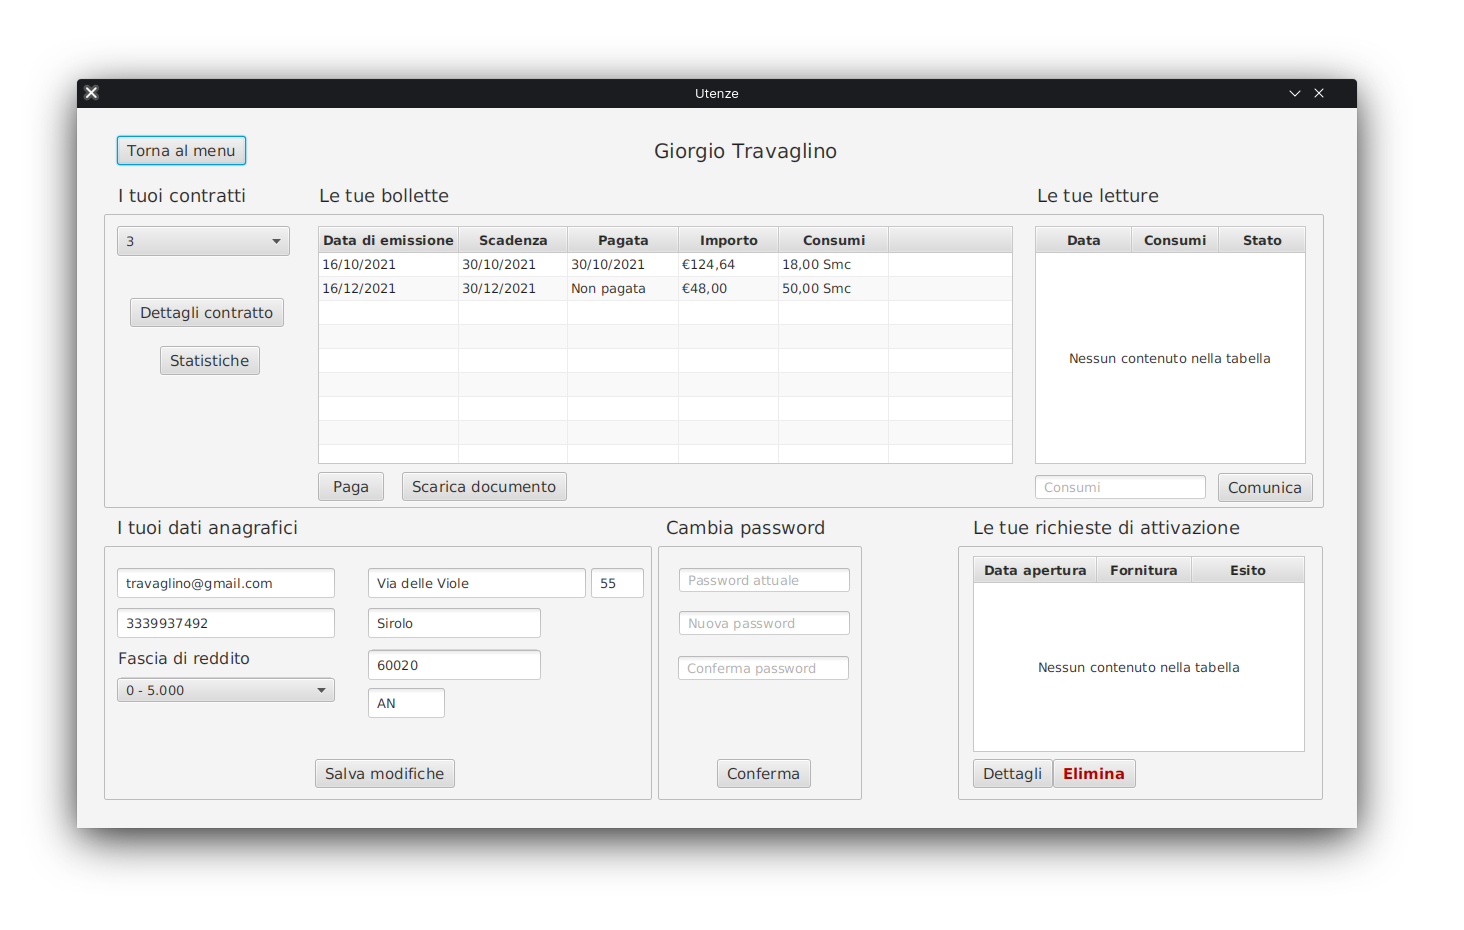
\includegraphics[width=1.1\textwidth]{images/user-area.png}}%
    \caption{Area clienti}
    \label{fig:user-area}
\end{figure}

L'inserimento di una richiesta di contratto (\cref{fig:sub-wizard}) avviene mediante una procedura guidata in cui l'applicazione verifica a ogni passaggio la correttezza dei dati, così da garantire la massima integrità del database. In qualsiasi momento è possibile tornare a una schermata precedente per apportare modifiche ai dati già inseriti. Nel caso in cui l'utente decida di interrompere anticipatamente la procedura, nessun dato verrà inserito nel database.

\begin{figure}[H]
    \centering{}
    \makebox[\textwidth][c]{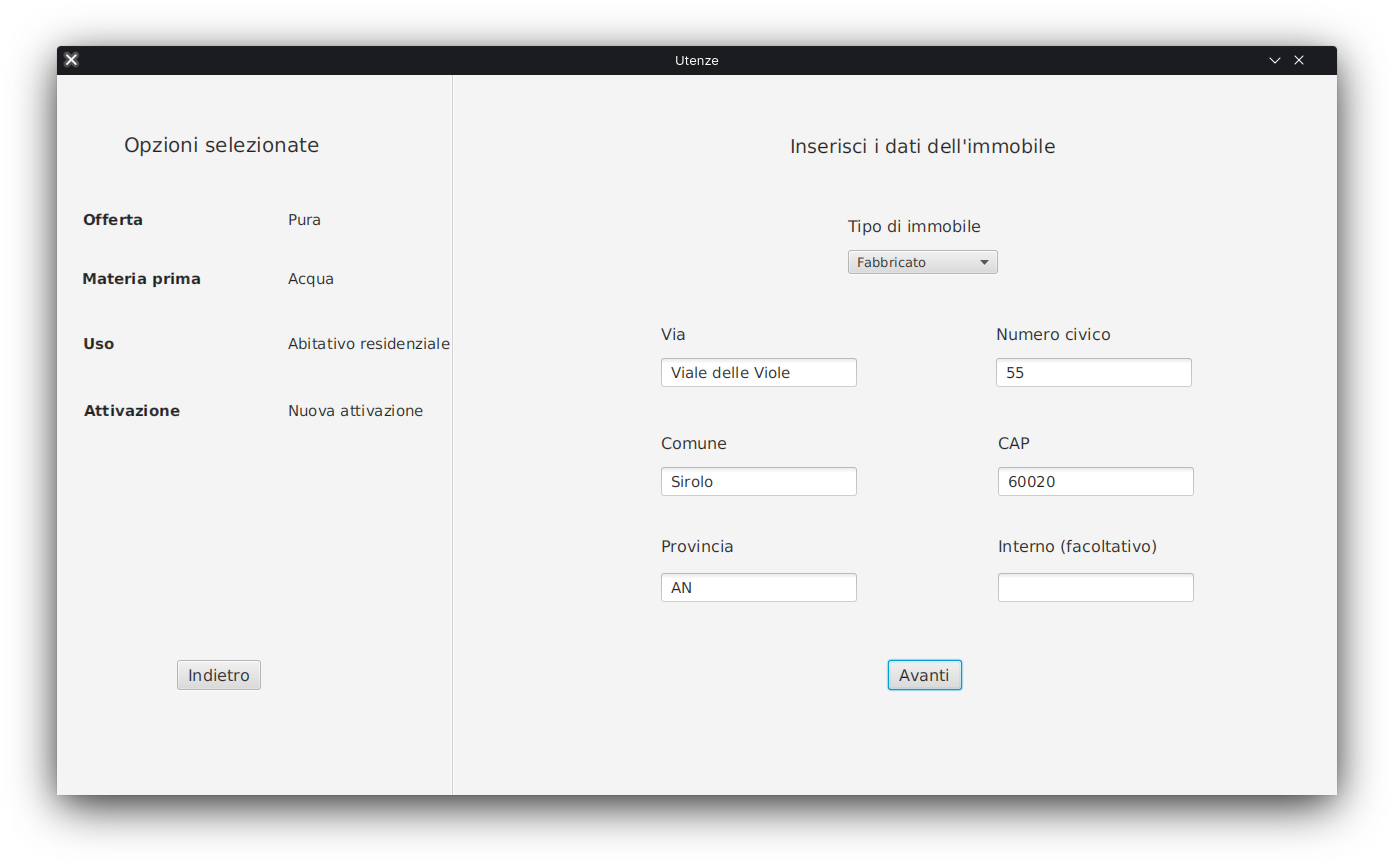
\includegraphics[width=1.1\textwidth]{images/sub-wizard.png}}%
    \caption{Creazione di una richiesta di contratto}
    \label{fig:sub-wizard}
\end{figure}

L'applicazione fornisce anche funzionalità non espressamente richieste nelle specifiche, come la possibilità filtrare i contratti in base allo stato dei pagamenti delle bollette (\cref{fig:sub-management}) o di aggiungere nuovi operatori.

\begin{figure}[H]
    \centering{}
    \makebox[\textwidth][c]{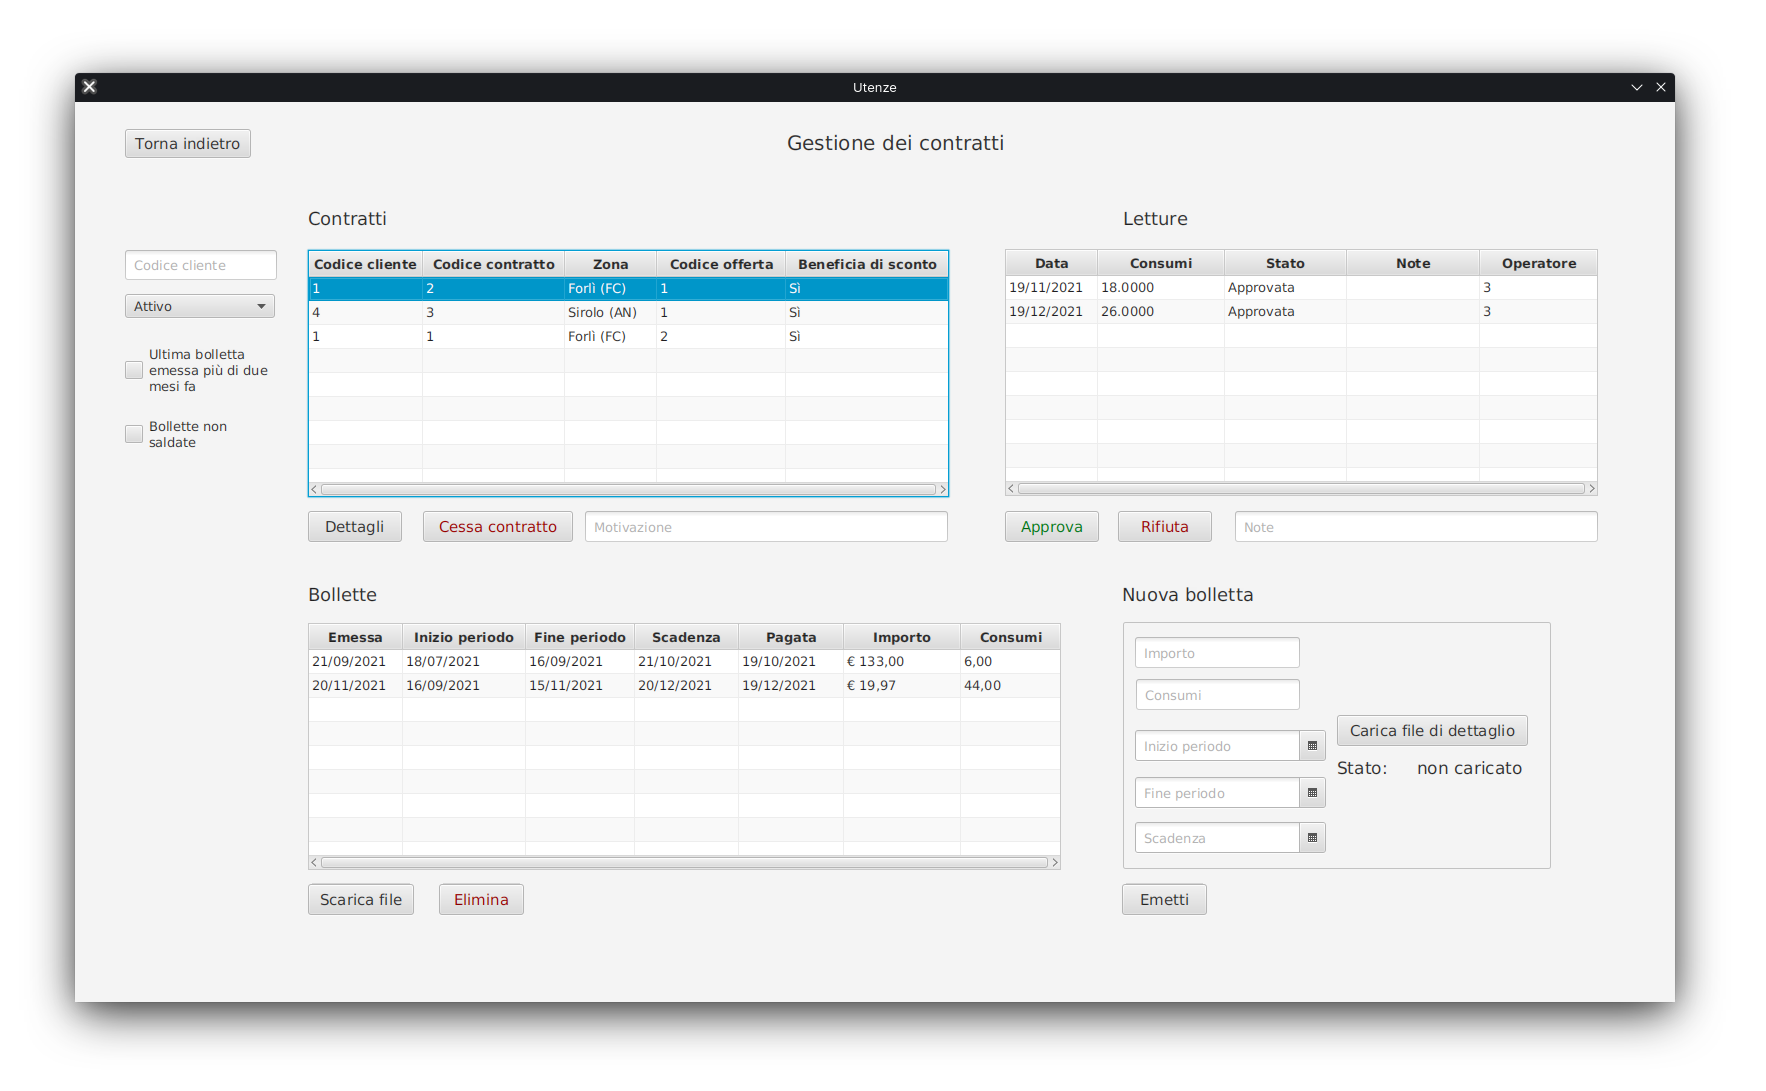
\includegraphics[width=1.2\textwidth]{images/sub-management.png}}%
    \caption{Gestione dei contratti}
    \label{fig:sub-management}
\end{figure}

\appendix
\chapter{Tabelle e viste in SQL}
\section{Creazione delle tabelle}
\begin{lstlisting}
create table bollette (
    NumeroBolletta integer auto_increment not null,
    DataEmissione date not null,
    DataInizioPeriodo date not null,
    DataFinePeriodo date not null,
    DataScadenza date not null,
    Importo decimal(20, 2) not null,
    Consumi decimal(20, 4) not null,
    DocumentoDettagliato mediumblob not null,
    IdOperatore integer not null,
    IdContratto integer not null,
    check (DataScadenza > DataEmissione),
    check (DataFinePeriodo > DataInizioPeriodo),
    constraint PK_BOLLETTA primary key (NumeroBolletta));
    
create table cessazioni (
    NumeroRichiesta integer not null auto_increment,
    DataAperturaRichiesta date not null,
    DataChiusuraRichiesta date default null,
    StatoRichiesta varchar(30) not null check (StatoRichiesta in ("In lavorazione", "Approvata", "Respinta")),
    NoteRichiesta varchar(500) not null,
    IdContratto integer not null,
    constraint PK_RIC_CESSAZIONE primary key (NumeroRichiesta));
    
create table clienti (
    CodiceCliente integer not null,
    FasciaReddito integer not null,
    constraint PK_CLIENTI primary key (CodiceCliente));

create table compatibilità (
    Offerta integer not null,
    Uso integer not null,
    constraint PK_COMPATIBILITÀ primary key (Offerta, Uso));
    
create table contatori (
    Matricola varchar(20) not null,
    MateriaPrima varchar(20) not null,
    IdImmobile integer not null,
    constraint PK_CONTATORI primary key (Matricola),
    constraint AK_CONTATORI unique (IdImmobile, MateriaPrima));

create table contratti (
    IdContratto integer not null auto_increment,
    DataAperturaRichiesta date not null,
    DataChiusuraRichiesta date default null,
    StatoRichiesta varchar(30) not null check (StatoRichiesta in ("In lavorazione", "Approvata", "Respinta")),
    NoteRichiesta varchar(500) not null,
    NumeroComponenti integer not null check (NumeroComponenti > 0),
    Uso integer not null,
    Offerta integer not null,
    TipoAttivazione integer not null,
    IdImmobile integer not null,
    IdCliente integer not null,
    constraint PK_CONTRATTO primary key (IdContratto));

create table immobili (
    IdImmobile integer not null auto_increment,
    Tipo varchar(20) not null check (Tipo = "Fabbricato" or Tipo = "Terreno"),
    Via varchar(50) not null,
    NumCivico varchar(10) not null,
    Interno varchar(10) not null default "",
    Comune varchar(50) not null,
    Provincia varchar(2) not null,
    CAP varchar(5) not null check (length(CAP) = 5),
    constraint TERRAIN_NO_UNIT check ((Tipo = "Terreno" and Interno = "") or (Tipo = "Fabbricato")),
    constraint IDIMMOBILE primary key (IdImmobile),
    constraint AK_IMMOBILE unique (Tipo, Via, NumCivico, Interno, Comune, Provincia, CAP));

create table letture (
    NumeroLettura integer auto_increment not null,
    MatricolaContatore varchar(20) not null,
    DataEffettuazione date not null,
    DataChiusuraRichiesta date default null,
    Stato varchar(30) not null check (Stato in ("In lavorazione", "Approvata", "Respinta")),
    Note varchar(500) not null,
    Consumi decimal(20, 4) not null check (Consumi >= 0),
    IdCliente integer not null,
    constraint PK_LETTURE primary key (NumeroLettura),
    constraint AK_LETTURE unique (MatricolaContatore, DataEffettuazione));

create table offerte (
    CodOfferta integer not null auto_increment,
    Nome varchar(20) not null,
    Descrizione varchar(1000) not null,
    CostoMateriaPrima decimal(10, 4) not null check(CostoMateriaPrima > 0.0),
    Attiva boolean not null default true,
    MateriaPrima varchar(20) not null,
    constraint PK_OFFERTA primary key (CodOfferta));

create table operatori (
    IdOperatore integer not null,
    Stipendio decimal(20, 2) not null check (Stipendio >= 0),
    constraint PK_OPERATORE primary key (IdOperatore));
    
create table `operatori contratti` (
    NumeroRichiesta integer not null,
    IdOperatore integer not null,
    constraint PK_OPCONTR primary key (NumeroRichiesta));
    
create table `operatori cessazioni` (
    NumeroRichiesta integer not null,
    IdOperatore integer not null,
    constraint PK_OPCONTR primary key (NumeroRichiesta));
    
create table `operatori letture` (
    Lettura integer not null,
    IdOperatore integer not null,
    constraint PK_OPCONTR primary key (Lettura));
    
create table pagamenti (
    NumeroBolletta integer not null,
    DataPagamento date not null,
    constraint PK_OPCONTR primary key (NumeroBolletta));

create table persone (
    IdPersona integer not null auto_increment,
    Nome varchar(50) not null,
    Cognome varchar(50) not null,
    CodiceFiscale varchar(16) not null,
    Via varchar(50) not null,
    NumCivico varchar(10) not null,
    Comune varchar(30) not null,
    CAP varchar(5) not null,
    Provincia varchar(2) not null,
    DataNascita date not null,
    NumeroTelefono varchar(10) not null,
    Email varchar(40) not null,
    Password varchar(30) not null check(length(Password) >= 8),
    constraint AK_PERSONA unique (Email),
    constraint PK_PERSONA primary key (IdPersona));
    
create table redditi (
    CodReddito integer not null,
    Fascia varchar(30) not null,
    Sconto decimal(7, 6) not null check (Sconto > 0.0 and Sconto <= 1.0),
    constraint PK_REDDITI primary key (CodReddito),
    constraint AK_REDDITI unique (Fascia));

create table `tipi attivazione` (
    CodAttivazione integer not null,
    Nome varchar(20) not null,
    Costo decimal(20, 2) not null,
    check(Costo >= 0),
    constraint PK_TIPO_ATTIVAZIONE primary key (CodAttivazione));

create table `tipologie uso` (
    CodUso integer not null auto_increment,
    Nome varchar(30) not null,
    StimaPerPersona decimal(20, 2) not null,
    ScontoReddito boolean not null,
    check(StimaPerPersona >= 0.0),
    constraint PK_USO_DEDICATO primary key (CodUso));

alter table bollette add constraint FK_CONTRATTO
    foreign key (IdContratto) references contratti (IdContratto);
     
alter table bollette add constraint FK_EMISSIONE
    foreign key (IdOperatore) references operatori (IdOperatore);
     
alter table cessazioni add constraint FK_RIFERIMENTO
    foreign key (IdContratto) references contratti (IdContratto);
     
alter table clienti add constraint FK_CODICECLIENTE
    foreign key (CodiceCliente) references persone (IdPersona);
     
alter table clienti add constraint FK_POSSEDIMENTO
    foreign key (FasciaReddito) references redditi (CodReddito);

alter table compatibilità add constraint FK_USOOFFERTA
    foreign key (Uso) references `tipologie uso` (CodUso) on delete cascade;

alter table compatibilità add constraint FK_OFFERTAUSO
    foreign key (Offerta) references offerte (CodOfferta) on delete cascade;

alter table contatori add constraint FK_INSTALLAZIONE
    foreign key (IdImmobile) references immobili (IdImmobile);
     
alter table contratti add constraint FK_RICHIESTA
    foreign key (IdCliente) references clienti (CodiceCliente);

alter table contratti add constraint FK_SOTTOSCRIZIONE
    foreign key (Offerta) references offerte (CodOfferta);

alter table contratti add constraint FK_USO
    foreign key (Uso) references `tipologie uso` (CodUso);

alter table contratti add constraint FK_ATTIVAZIONE_TRAMITE
    foreign key (TipoAttivazione) references `tipi attivazione` (CodAttivazione);

alter table contratti add constraint FK_COLLEGAMENTO
    foreign key (IdImmobile) references immobili (IdImmobile);

alter table letture add constraint FK_CORRISPONDENZA
    foreign key (MatricolaContatore) references contatori (Matricola) on update cascade;
     
alter table letture add constraint FK_EFFETTUAZIONE
    foreign key (IdCliente) references clienti (CodiceCliente);
     
alter table operatori add constraint FK_DATIANAGRAFICI
    foreign key (IdOperatore) references persone (IdPersona);
    
alter table `operatori cessazioni` add constraint FK_GESTIONE_CC1
    foreign key (NumeroRichiesta) references cessazioni (NumeroRichiesta) on delete cascade;
    
alter table `operatori cessazioni` add constraint FK_GESTIONE_CO1
    foreign key (IdOperatore) references operatori (IdOperatore) on delete cascade;

alter table `operatori contratti` add constraint FK_GESTIONE_CC2
    foreign key (NumeroRichiesta) references contratti (IdContratto) on delete cascade;
    
alter table `operatori contratti` add constraint FK_GESTIONE_CO2
    foreign key (IdOperatore) references operatori (IdOperatore) on delete cascade;

alter table `operatori letture` add constraint FK_GESTIONE_LC
    foreign key (Lettura) references letture (NumeroLettura) on delete cascade;
    
alter table `operatori letture` add constraint FK_GESTIONE_LO
    foreign key (IdOperatore) references operatori (IdOperatore) on delete cascade;

alter table pagamenti add constraint FK_PAGAMENTO
    foreign key (NumeroBolletta) references bollette (NumeroBolletta);
\end{lstlisting}

\section{Creazione delle viste}
\begin{lstlisting}
create view `clienti dettagliati` as
select P.*, C.FasciaReddito
from persone P, clienti C
where P.IdPersona = C.CodiceCliente;
 
create view `operatori dettagliati` as
select P.*, O.Stipendio
from persone P, operatori O
where P.IdPersona = O.IdOperatore;
   
create view `richieste contratto` as
select IdContratto, DataAperturaRichiesta, DataChiusuraRichiesta, StatoRichiesta, NoteRichiesta, NumeroComponenti, Uso, Offerta, TipoAttivazione, IdImmobile, IdCliente
from contratti
where DataChiusuraRichiesta is null or (DataChiusuraRichiesta is not null and StatoRichiesta = "Respinta");
   
create view `contratti approvati`
as select C.*
from contratti C
where C.DataChiusuraRichiesta is not null and C.StatoRichiesta = "Approvata";
                                      
create view `contratti attivi`
as select C.*
from `contratti approvati` C
where not exists (select E.NumeroRichiesta
                from cessazioni E
                where E.IdContratto = C.IdContratto
                and E.DataChiusuraRichiesta is not null
                and E.StatoRichiesta = "Approvata");
\end{lstlisting}

\end{document}
